\documentclass[a4paper]{report}

\usepackage[utf8]{inputenc}

\usepackage{amsfonts}
\usepackage{amsmath}

\usepackage{graphicx}
\usepackage{subcaption}

\usepackage{url}
\usepackage{hyperref}

\usepackage{gensymb}

\usepackage[square,sort,comma,numbers]{natbib}
\usepackage{pdfpages}

\usepackage{listings}
\usepackage{color}

% preamble

\definecolor{comments}{rgb}{0.4, 0.4, 0.4}
\renewcommand{\ttdefault}{pcr}

\lstset{
  language=Java,
  tabsize=2,
  basicstyle=\footnotesize\ttfamily,
  keywordstyle=\bfseries,
  commentstyle=\itshape\color{comments},
  frame=single,
  numbers=none,
  breakatwhitespace=true,
  breaklines=true,
  keepspaces=false,
  rangeprefix=/*---,
  rangesuffix=---*/,
  includerangemarker=false,
  columns=fullflexible,
  firstnumber=auto,
  literate={private}{}1 {protected}{}1
}

\lstdefinestyle{inline}{
  frame=L,
  numbers=none
}

%%% start lstinputlistings
% Taken from
% http://tex.stackexchange.com/questions/48903/how-to-extend-the-lstinputlisting-command

\newlength{\rawgobble}
\newlength{\gobble}
\newlength{\gobblea}

% The width of a single space. basicstyle from lstset should be used
\sbox0{\Huge\ttfamily \ }

% Remove a single space
\settowidth{\rawgobble}{\Huge\ttfamily \ }
\setlength{\rawgobble}{-\rawgobble}

\makeatletter
\def\sepstar#1*#2\relax{%
    \def\sepstarone{#1}%
    \def\sepstartwo{#2}%
}
\lst@Key{firstlineandnumber}\relax{\def\lst@firstline{#1\relax}\def\lst@firstnumber{#1\relax}}
\lst@Key{widthgobble}{0*0}{
    % Reindent a bit by multiplying with 0.9,
    % then multiply by tabsize and number of
    % indentation levels
    \sepstar #1\relax
    \setlength{\gobble}{0.9\rawgobble}
    \setlength{\gobble}{\sepstarone\gobble}
    \setlength{\gobble}{\sepstartwo\gobble}
    \setlength{\gobblea}{\gobble}
    \addtolength{\gobblea}{10pt}
    \def\lst@xleftmargin{\gobble}
    \def\lst@framexleftmargin{\gobble}
    \def\lst@numbersep{\gobblea}
}
\makeatother

%%% end lstinputlistings

\newcommand{\inlinecode}[1]{{\footnotesize\texttt{#1}}}
\newcommand{\todo}[1]{\textcolor{red}{\textbf{To Do:} #1}}

% content
\begin{document}

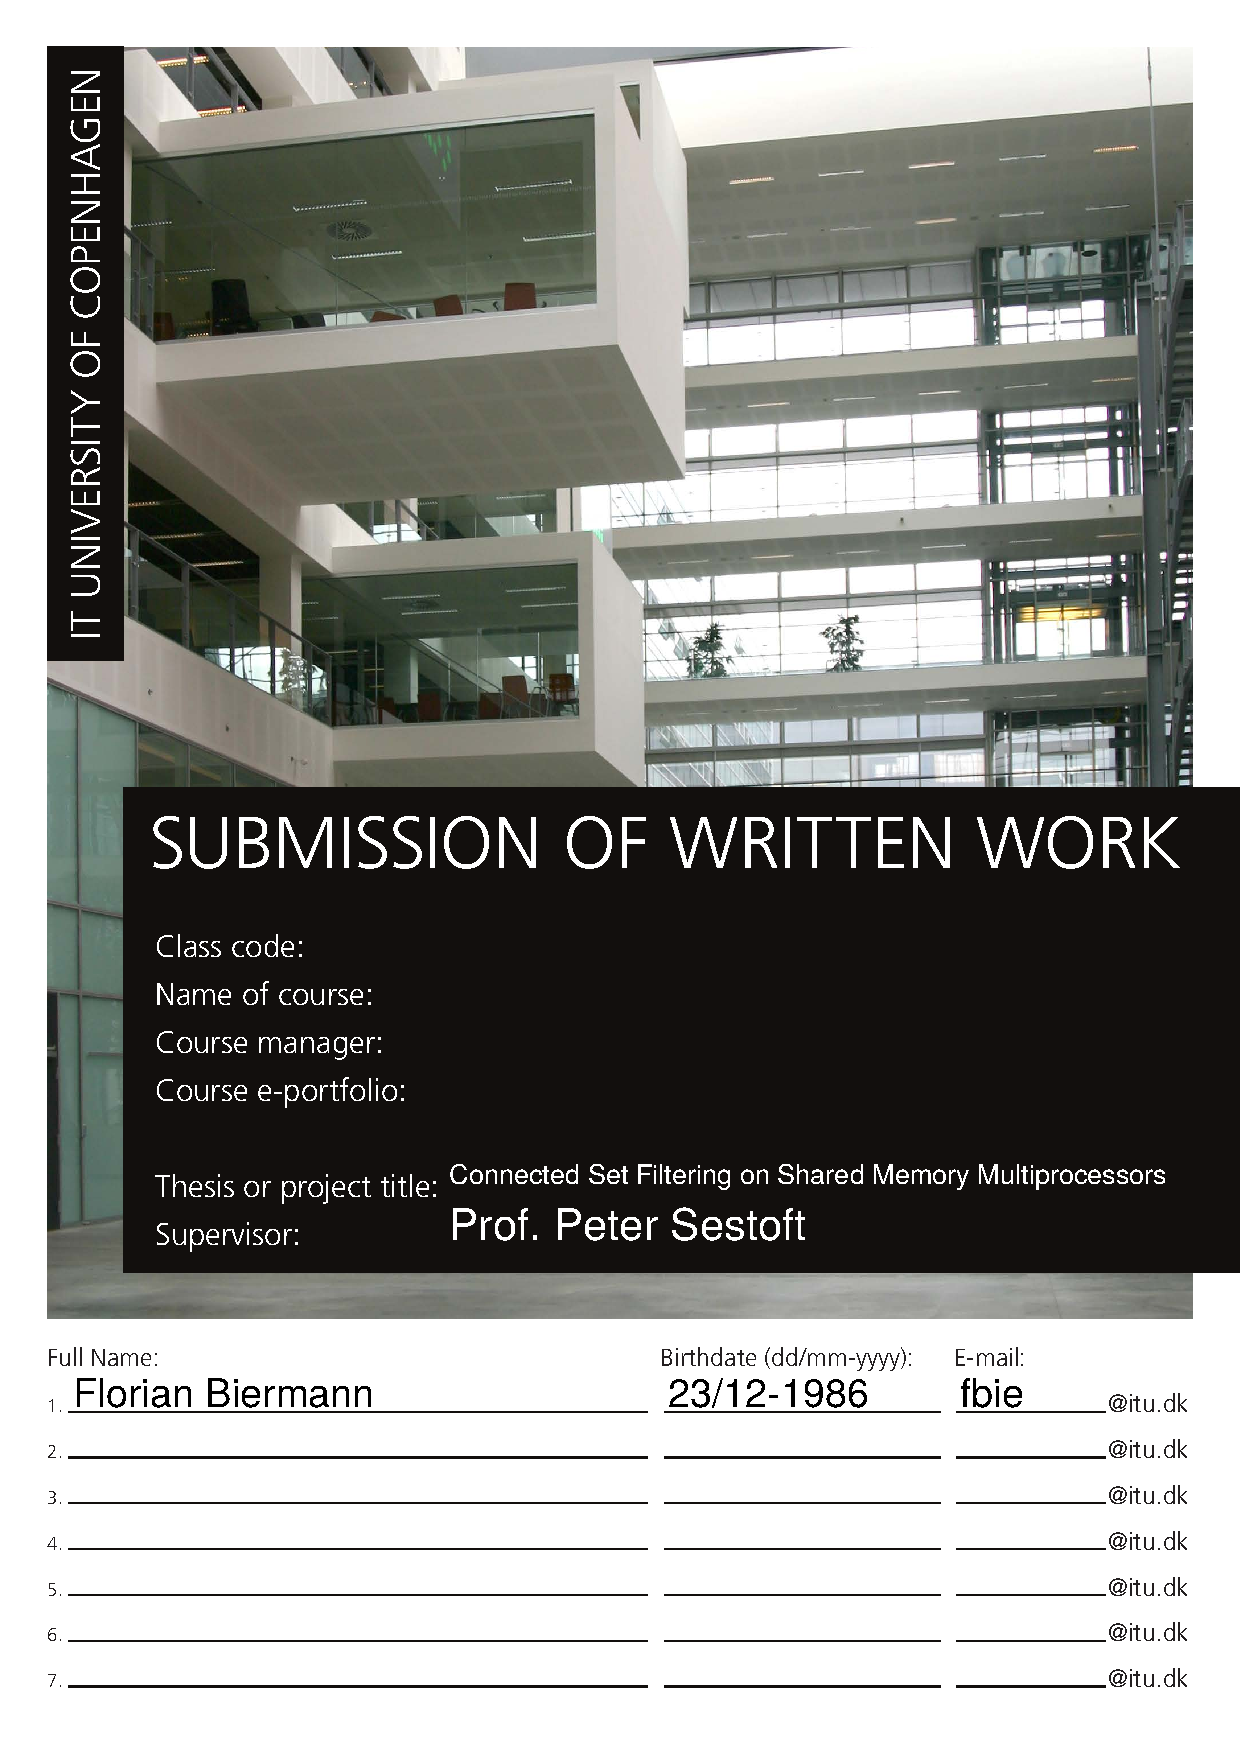
\includepdf[pages={1}]{itu-frontpage.pdf}

\newpage

~ % Purposly empty
\thispagestyle{empty}

\newpage

\begin{titlepage}
  \begin{center}
    \vspace*{1cm}

    {\LARGE \textbf{Connected Set Filtering on Shared Memory Multiprocessors}}

    \vspace{1.5cm}

    Submitted in partial fulfillment of the requirements\\
    towards the M.Sc. degree

    \vspace{0.8cm}

    by\\

    \vspace{0.8cm}

    {\Large \textbf{Florian Biermann}}\\
    \texttt{fbie@itu.dk}

    \vfill

    IT University of Copenhagen\\
    Denmark

    \vspace{0.8cm}

    The research work in this thesis has been carried out\\
    under the supervision of Prof. Peter Sestoft.

    \vspace{1.5cm}

    June 2, 2014

  \end{center}
\end{titlepage}

\pagenumbering{roman}

\newpage

~ % Purposly empty
\thispagestyle{empty}

\newpage

\begin{abstract}
  This thesis reports on the development of a family of parallel algorithms for
  computing area openings and closings on gray-scale images, in order to
  increase performance on large images. Previous parallel and sequential
  algorithms did not fully exploit the parallel nature of contemporary
  computers. The novelty in this thesis is that the developed algorithms use
  variants of a shared union-find data structure. This shared union-find
  approach reduces the amount of sequential work substantially.

  By conducting structured performance experiments, I show that, in particular,
  a certain type of the new, parallel algorithms outperforms the original,
  sequential algorithm by far on large images. Moreover, by identifying formal
  correctness properties and by using Java Pathfinder to model check the
  respective implementations, I show that the new parallel algorithms are
  formally correct. Additionally, I discuss the feasibility of model checking
  complex image filtering algorithms.

  Throughout the thesis, I review different variants of concurrent union-find
  and asses their performance on random graphs, as well as their adaption to
  parallel area opening. The presented results show that the structure of random
  input graphs has a greater influence on performance than their mere
  size. Furthermore, I discuss input image structure in relation to the
  performance, exhibited by the various parallel area opening
  algorithms. Performance experiments show that performance limitations on
  random graphs do not necessarily apply to the performance on images. This
  thesis opens up for many future research directions on parallel morphological
  algorithms.
\end{abstract}

%%% Local Variables:
%%% mode: latex
%%% TeX-master: "main"
%%% End:


\newpage

~ % Purposly empty
\thispagestyle{empty}

\newpage

\tableofcontents

\listoffigures

\listoftables

\newpage

~ % Purposly empty

\newpage

\newcommand{\synthone}{area-open-14-05-14-18-25-15-fbie@mtlab-synth001_large_jpg-3000-10}
\newcommand{\synthtwo}{area-open-14-05-14-18-25-15-fbie@mtlab-synth002_large_jpg-3000-10}

\newcommand{\synththreea}{area-open-14-05-14-13-01-07-fbie@mtlab-synth003_large_jpg-3000-10}
\newcommand{\synththreeb}{area-open-14-05-15-12-14-54-fbie@dolab-synth003_large_jpg-6000-10}
\newcommand{\synththreec}{area-open-14-05-16-12-28-50-fbie@dolab-synth003_large_jpg-9000-10}

\newcommand{\synthfour}{area-open-14-05-13-17-33-25-fbie@dolab-synth004_large_jpg-3000-10}
\newcommand{\synthfive}{area-open-14-05-14-18-23-10-fbie@dolab-synth005_large_jpg-3000-10}

\newcommand{\pixel}{area-open-14-04-23-09-11-21-fbie@dolab-synth004_jpg-1500-10}

\newcommand{\natone}{area-open-14-05-02-11-45-18-fbie@dolab-natural001_large_jpg-1500-10}
\newcommand{\nattwo}{area-open-14-04-23-09-11-21-fbie@dolab-natural002_jpg-1500-10}
\newcommand{\natthree}{area-open-14-04-23-09-11-21-fbie@dolab-natural003_jpg-1500-10}

\newcommand{\plotdata}[1]{-d#1}
\newcommand{\plotinclude}[1]{-i#1}
\newcommand{\plotremove}[1]{-r#1}

\newcommand{\ms}{\plotdata{ms}}
\newcommand{\retries}{\plotdata{retries}}
\newcommand{\cache}{\plotdata{cache-misses}}
\newcommand{\instructions}{\plotdata{instructions}}
\newcommand{\gc}{\plotdata{gc}}
\newcommand{\prefetches}{\plotdata{prefetches}}

\newcommand{\opt}{\plotinclude{opt}\plotremove{array|bucket}}
\newcommand{\stm}{\plotinclude{stm}\plotremove{array|bucket}}

\newcommand{\plotsingle}[3]
{
  \begin{subfigure}{0.55\textwidth}
    \includegraphics[width=\textwidth]{plots/#1.pdf}
    \caption{#2}
    \label{fig:#3}
  \end{subfigure}
}

\newcommand{\plotrow}[6]
{
  \makebox[\textwidth][c]{
    \plotsingle{#1}{#2}{#3}
    \plotsingle{#4}{#5}{#6}
  } %makebox
}

\newcommand{\unionfindplotlow}[1]
{
  \plotrow
  {union-find-14-04-08-14-23-26-fbie@dolab-n500000_p0_000001_gr-10-d#1}
  {\emph{low-low}}
  {uf-results-#1-low-low}
  {union-find-14-04-08-14-23-26-fbie@dolab-n500000_p0_000005_gr-10-d#1}
  {\emph{low-high}}
  {uf-results-#1-low-high}
}

\newcommand{\unionfindplothigh}[1]
{
  \plotrow
  {union-find-14-04-08-14-23-26-fbie@dolab-n1000000_p0_000005_gr-10-d#1}
  {\emph{high-low}}
  {uf-results-#1-high-low}
  {union-find-14-04-08-14-23-26-fbie@dolab-n1000000_p0_00001_gr-10-d#1}
  {\emph{high-high}}
  {uf-results-#1-high-high}
}

\newcommand{\areaopenplotpixels}
{
  \plotrow
  {\pixel\ms\plotinclude{pixel}}
  {Duration in milliseconds.}
  {pixel-queues-ms}
  {\pixel\retries\plotinclude{pixel}}
  {Number of re-tries.}
  {pixel-queues-retries}

  \plotrow
  {\pixel\cache\plotinclude{pixel}}
  {Number of cache misses.}
  {pixel-queues-cache-misses}
  {\pixel\instructions\plotinclude{pixel}}
  {Number of issued CPU instructions.}
  {pixel-queues-instructions}
}

\newcommand{\fullrow}[3]
{
  \plotrow
  {#1\plotdata{#2}\opt}
  {Optimistic}
  {#3-opt-#2}
  {#1\plotdata{#2}\stm}
  {STM}
  {#3-stm-#2}
}

\newcommand{\fullmsrow}[2]
{
  \fullrow{#1}{ms}{#2}
}

\newcommand{\fullrawrow}[3]
{
  \plotrow
  {raw/#1\plotdata{#2}\plotinclude{opt}}
  {Optimistic}
  {#3-opt-#2}
  {raw/#1\plotdata{#2}\plotinclude{stm}}
  {STM}
  {#3-stm-#2}
}

\newcommand{\fullrawrownat}[3]
{
  \plotrow
  {raw/#1\plotdata{#2}\plotinclude{opt}\plotremove{pixel}}
  {Optimistic}
  {#3-opt-#2}
  {raw/#1\plotdata{#2}\plotinclude{stm}\plotremove{pixel}}
  {STM}
  {#3-stm-#2}
}


%%% Local Variables:
%%% mode: latex
%%% TeX-master: "main"
%%% End:


\pagenumbering{arabic}

\chapter{Introduction}
\label{chpt:introduction}

Over recent years, the quality and average size of digital images has increased
tremendously. Additionally, the mere count of digital images produced every day
is increasing, too. There are various reasons to analyze digital images
automatically, for example in the medical domain. Here, modern clinical scans,
such as magnetic resonance tomography (MRT) or computing tomography (CT),
produce huge amounts of data. In order to speed up the analysis of such huge
images, there has always been a trend to parallelize image analysis algorithms,
as some of the problems on images are embarrassingly parallel. Nevertheless,
there are also operations on images that are hard to parallelize, because the
possibilities for parallelism are not obvious. One of these operations is
morphological filtering.

Morphological filters are operators on two or three dimensional
images that filter connected components from the input image. They are defined
in terms of openings and closings, where an opening removes bright regions from
an image while a closing removes dark regions \cite{Serra1992Overview}.

More complex, shape preserving morphological filters are \emph{area opening and
  closing} (I will refer to these filters as \emph{area opening} through the
rest of this thesis). Given a minimum area parameter $\lambda$, all bright or
dark elements respectively of size less than $\lambda$ are removed
\cite{Vincent1994Morphological}. Area opening is useful for image segmentation
and noise removal. There already exist a number of algorithms to compute area
opening, differing tremendously in performance \cite{Vincent1994Morphological,
  Wilkinson2000Fast, Meijster2002Comparison}. These three algorithms are all
implemented sequentially.

In this thesis, I report on the development of a family of parallel algorithms
for area opening for the sake of increased performance on large
images. \citet{Wilkinson2008Concurrent} developed a parallel algorithm to
compute morphological attribute filters, a generalization of morphological area
filtering, using Max-Trees. However, it consists of a major sequential part
\cite{Wilkinson2008Concurrent}. The novelty in this thesis is that the
algorithms presented here are based on the union-find area opening algorithm by
\citet{Meijster2002Comparison} and use variants of a shared union-find data
structure \cite{Tarjan1983Data} in order to reduce the amount of sequential work
substantially. I will show that some of the new parallel algorithms can
outperform the original, sequential algorithm and also that the new parallel
algorithms are formally correct.

Throughout this thesis, I use valid Java code to describe algorithms, except
where stated otherwise. For brevity, some less important implementation details
may be omitted. These are replaced by descriptive comments.

\section{Contributions}
\label{sec:introduction-contributions}

The parallel algorithms, that I developed in this thesis, are based on the
union-find based area opening algorithm by \citet{Meijster2002Comparison}. To
fully exploit parallelism, it is therefore important to address shared
union-find data structures. Concurrent union-find data structures have already
been subject of research \cite{Berman2010Multicore, Anderson1994Waitfree}.

The contributions of this thesis are the following:

\begin{itemize}
\item Reviewing concurrent union-find data structures, their performance and how
  they can be applied to our problem. Not all union-find algorithms directly map
  to area opening. Dedicated performance experiments provide us with insights
  into which algorithm best fits our needs.

\item Developing and evaluating a number of parallel algorithms for
  morphological area opening. I will evaluate algorithms in terms of performance
  and provide a set of repeatable experiments that show how the algorithms
  behave, given certain input over a range of processors to run on.

\item Verifying the correctness of the improved algorithm using Java Pathfinder
  \cite{Visser2003Model}. Even though experimental testing can increase
  confidence, the inherent non-determinism of thread scheduling and delays in
  parallel programs makes it strictly speaking impossible to test all possible
  execution branches. Therefore, I show the correctness of the parallel area
  opening algorithms by more formal methods.
\end{itemize}

\section{Programming Shared Memory Multiprocessors}
\label{sec:introduction-concurrency}

Software for shared memory multiprocessors has been subject of research for a
long time already \cite{Herlihy2008Art}. Yet, programming concurrent and
parallel applications, especially with low-level synchronization primitives, has
not hit the main stream entirely yet \cite{Herlihy2008Art}. In this section, I
will give a brief overview over the basics of programming for shared memory
multiprocessors.

\subsection{Blocking Programs}
\label{sec:introduction-blocking}

Blocking parallelism describes programs where independent processes, or threads,
wait for each other in order to make progress \cite{Herlihy2008Art}. This
waiting is achieved by the use of locks, which protect resources from concurrent
access.

In such a program, a thread $A$ has to wait, while thread $B$ holds the lock to a
resource $R$. As soon as $B$ releases the lock, $A$ can attempt to acquire the
lock for $R$, blocking $B$ from accessing $R$ \cite{Herlihy2008Art}. This scheme
can result in deadlocks ($A$ waiting indefinitely for $B$ to release the lock or
vice versa), if access to the shared resource via locking is not implemented
consistently or, if a thread terminates unexpectedly while holding the lock, thus
never being able to release it again. Also, waiting threads cannot make any
progress while the resource is locked, such that precious computing time goes
wasted \cite{Herlihy2008Art}.

One can not only block resource access, but also principal progress, using
barriers. Barriers typically block the progress of each thread, that reached the
barrier, until all other threads also arrived at this point in the code. Only
then all threads are allowed to continue together \cite{Herlihy2008Art}.

\subsection{Lock-Free and Wait-Free Programs}
\label{sec:introduction-wf-primitives}

Lock-free and wait-free programs are closely related. The wait-free property is
stronger than the lock-free property: lock-free algorithms are defined by the
absence of locks, while wait-free algorithms are guaranteed to terminate in a
bounded number of steps \cite{Alistarh2013Are} with all threads \emph{always}
making progress.

Theoretically, wait-free algorithms outperform lock-free algorithms, but recent
research by \citet{Alistarh2013Are} suggests that lock-free programs in practice
actually exhibit wait-free performance. Their results suggest, that constructing
extremely complex, wait-free algorithms might be unnecessary
\cite{Alistarh2013Are}.

Lock- and wait-free algorithms perform in general much better in comparison to
lock-based algorithms. To be able to update values and references consistently,
there exist synchronization primitives as CPU instructions, which, in Java, are
exposed to the programmer as function calls on container types.

\subsubsection{Compare and Swap}
\label{sec:introduction-cas}

The compare-and-swap (\emph{CAS}) primitive atomically, i.e. as a single
instruction on the CPU, performs the equivalent to the following code (here
denoted in C{}\verb!++!) \cite{Goetz2006Java, Herlihy2008Art}:

\begin{lstlisting}[frame=L, language=C++]
  template <typename T>
  bool CAS(T* r, const T& e, const T& n)
  {
    if (*r == e) {
      *r = n;
      return true;
    }
    return false;
  }
\end{lstlisting}

Given a pointer to some variable \inlinecode{r}, a reference to an expected
value of the same type \inlinecode{e}, and a replacement value \inlinecode{n},
the primitive replaces the value, which \inlinecode{r} points to, only, if
\inlinecode{r} points to \inlinecode{e} at the time of the call. \emph{CAS}
returns a boolean to the caller, indicating, whether the update was
successful. The caller can then react to the failure, for example by simply
updating its local copy of the value and re-trying the operation until it
succeeds.

Essentially, the caller only can update a variable if he is up-to-date with its
latest value \cite{Goetz2006Java}. This control structure can be used to build
entire data structures, as we will see next. A major issue is the lack of
composition, meaning that it is impossible to update two or more independent
variables atomically \cite{Herlihy2008Art}.

Java does not pass values by pointer, so the value of a function parameter
cannot be changed globally by a function. Therefore, Java implements \emph{CAS}
through the \inlinecode{AtomicReference} class, which references some object
internally. Its public member function \inlinecode{compareAndSet} corresponds to
\emph{CAS} \cite{Goetz2006Java}. Java also provides multiple specialized atomic
data types, like for instance \inlinecode{AtomicInteger} or
\inlinecode{AtomicLong}, as well as array variants of those types
\cite{Goetz2006Java}.

\subsubsection{Michael-Scott Queue}
\label{sec:introduction-msq}

A well known wait-free data structure is the \citet{Michael1996Simple} queue
(\emph{MSQ}). The \emph{MSQ} is a first-in-first-out queue, using only the
compare-and-swap primitive to synchronize between threads that concurrently
access it.

Internally, the \emph{MSQ} maintains two pointers to the \inlinecode{head} and
the \inlinecode{tail} of a linked list, where the \inlinecode{head} always is a
dummy node. By checking the state of the next pointer of the \inlinecode{tail}
and the \inlinecode{head} node, the algorithm can figure out, whether some
thread currently is executing an update on the queue. If that is the case, all
threads work towards maintaining consistency on the queue. If not, a new update
can be initiated. This pattern makes the \emph{MSQ} wait-free and prone to
unexpected thread termination \cite{Michael1996Simple, Goetz2006Java}. The
\inlinecode{ConcurrentLinkedQueue} class provides an \emph{MSQ} based
implementation in the JVM.

\subsection{Transactional Memory}
\label{sec:introduction-transm}

Transactional memory is a concept borrowed from relational data bases, where
consistency is the most important property. In data base systems, a transaction
is a concatenation of modifications that only commit (i.e. become permanent), if
no other changes have been made to the data touched by this transaction, since
it began \cite{Herlihy2008Art}.

When applied to shared memory multiprocessors, concurrent threads issue a
transaction for any number of memory modifications they want to perform
atomically. Equally, these transactions only commit, if there are no conflicts
due to other threads writing to the same memory locations. Otherwise, the
changes get rolled back and the transaction, depending on the re-try policy of
the system, can be re-tried or simply aborted \cite{Herlihy2008Art}.

From the outside, a transaction is seen as a single atomic update of multiple
variables. This is a huge advantage compared to \emph{CAS}. Also, it reduces
complexity, since the synchronization is entirely transparent to the programmer
\cite{Herlihy2008Art}. Today's main-stream hardware does not support
transactional memory. Instead, software transactional memory (\emph{STM}) has
been subject to research, originally proposed by Shavit et
al. \cite{Shavit1997Software, Herlihy2008Art}.

Neither OpenJDK nor the Oracle JVM implement transactional memory. Instead,
there exist a number of \emph{STM} libraries for Java. The code for this thesis
uses the \emph{multiverse} library, which is open source and freely available
\cite{MultiverseWebsite}. The algorithms presented in this thesis use
\emph{multiverse} as a black-box to gain access to transactional memory
capabilities. Therefore, I will not provide a detailed description of \emph{STM}
algorithms. Further information on the implementation details of
\emph{multiverse} can be found on the library's website
\cite{MultiverseWebsite}.

%%% Local Variables:
%%% mode: latex
%%% TeX-master: "main"
%%% End:


\chapter{Mathematical Morphology}
\label{chpt:morphology}

This chapter introduces the notion of mathematical morphology, reflects on its
formalism and details the special case of morphological area opening. We will
take a look at use cases and show the effects of area opening on 2D images. The
chapter concludes with the introduction of the algorithm, which is the basis for
the algorithms developed in this thesis.

Sections~\ref{sec:morphology-area-opening} and \ref{sec:morphology-examples} are
based on a previous project I conducted \cite{Biermann2013Morphological}. The
contents are corrected and cut down to the most relevant parts, for brevity.

\section{Morphological Area Opening}
\label{sec:morphology-area-opening}

This section briefly outlines the formalism of morphological area opening. I
will not go into the details of lattice theory and the foundations of
mathematical morphology. A good reference point for the interested reader is
\emph{An overview of morphological filtering} by \citet{Serra1992Overview}.

Mathematical morphology is, intuitively speaking, the formal study of
shapes. Morphological filters operate on partially ordered sets. Therefore,
morphology only applies to single-channel images, as their elements
(i.e.~pixels) can be ordered by their height (i.e.~gray-scale value)
\cite{Serra1992Overview}. While morphological filtering can also be performed on
binary images, I will omit this case. Computing morphological area openings on
binary images is trivial and reduces to flat component labeling.

Two elementary operations in mathematical morphology are \emph{dilation},
denoted $\delta$, and \emph{erosion}, denoted $\epsilon$, which are mathematical
duals. They are digitally implemented using a structuring element, for example a
disk, a square or a hexagon. Intuitively, erosion extends dark components of an
image, by moving the structuring element around their outer borders. Dilation
does the opposite, narrowing dark elements, by moving the structuring element on
the inner border of the component. The concatenation of both, $\gamma = \epsilon
\circ \delta$, produces the morphological opening of an image. Closing, the
respective dual, is defined as $\varphi = \delta \circ \epsilon$
\cite{Serra1992Overview}. As already pointed out in
chapter~\ref{chpt:introduction}, we will for the remainder only focus on
morphological openings, since area opening and closing are mathematical duals:
computing area opening on an inverted image and inverting the result again,
corresponds to computing area closing \cite{Wilkinson2000Fast}.

Computing the morphological opening of an image $I$, for a structuring element
$S$, removes all bright components from $I$, that do \emph{not} resemble the
shape of $S$ \cite{Serra1992Overview}. This essentially means that, in order to
separate information from the image (i.e. to perform segmentation), we are
required to provide concrete, a priori, non-parametric knowledge
\cite{Vincent1994Morphological}, which sometimes is not available or not
applicable. To work around this problem, a union of multiple openings with
different structuring elements can be constructed, at the cost of filtering an
image repeatedly.

To provide more general means of filtering connected components from an image,
\citet{Vincent1994Morphological} introduced \emph{morphological area opening},
denoted as $\gamma^a_{\lambda}$. In contrast to classical morphological opening,
area opening is performed with a parameter of \emph{area}, or size, called
$\lambda$. One can see area opening as classical morphological opening with a
dynamically shaped structuring element, that adjusts to the structure of the
image and grows up to a certain size. All bright components of an image of size
less than $\lambda$ are removed in its area opening
\cite{Vincent1994Morphological}. Section~\ref{sec:morphology-examples} details
the effects of morphological area opening.

Let an image be represented by a function $f: I \rightarrow \mathbb{R}^*, I
\subset \mathbb{R}^2$. Let, moreover, $T_h(x) \subseteq I, x \in I$ be the
connected component to which $x$ belongs at some gray-value threshold level
$h$. Also, let $\left\vert{}\right\vert$ denote set cardinality. Then, area
opening is defined by \cite{Vincent1994Morphological}:

\begin{equation}
  \gamma^a_{\lambda}(f)(x) = sup\{h \leq f(x) \vert ~ \left\vert{T_h(x)}\right\vert \geq \lambda \}
\end{equation}

This is essentially incremental region-growing for each gray-level threshold of
the input image \cite{Vincent1994Morphological}. This formalism can directly be
projected onto code, resulting in very poor performance, however. A number of
more efficient algorithms have been conceived, which are outlined in the
following section~\ref{sec:morphology-algorithm}.

\section{Usage Example}
\label{sec:morphology-examples}

Typically, area opening is used to either remove unwanted elements, like noise,
from an image, or to identify objects in a scene. Vincent originally proposed to
use area opening to identify micro-aneurysms in images of eye blood-vessels
\cite{Vincent1994Morphological}. One would first compute the area opening of the
image for some $\lambda$, which corresponds to the expected size of aneurysms in
pixels. To identify the location of the aneurysms, it is enough to compute the
pixel-wise difference between the original image and its area opening.

This approach can be used in many different settings. Morphological area opening
has been used in literature for the segmentation of red blood cells in the case
of automated Malaria diagnosis \cite{MohanaRao2001Areagranulometry,
  Tek2010Parasite}. In figure~\ref{fig:morphology-examples-malaria-orig}, we can
see an image of human red blood cells ($800 \times 600$ pixels), infected with
Malaria parasites. The successive images,
\ref{fig:morphology-examples-malaria-1500} through
\ref{fig:morphology-examples-malaria-4500}, show the area closing of the source
image for increasing values of $\lambda$ in pixels. We use area closing here,
because the blood cells are darker than the background. Alternatively, one can
simply compute the negative of the image before and after opening it
\cite{Wilkinson2000Fast}. The bigger $\lambda$ gets, the more cells are removed
from the image, while the background remains unmodified. By those means, we are
able to compute an approximation of the background model, which is helpful for
separating the single blood cells from the image background.

\begin{figure}
  \centering

  \makebox[\textwidth][c]{

    \begin{subfigure}{0.25\textwidth}
      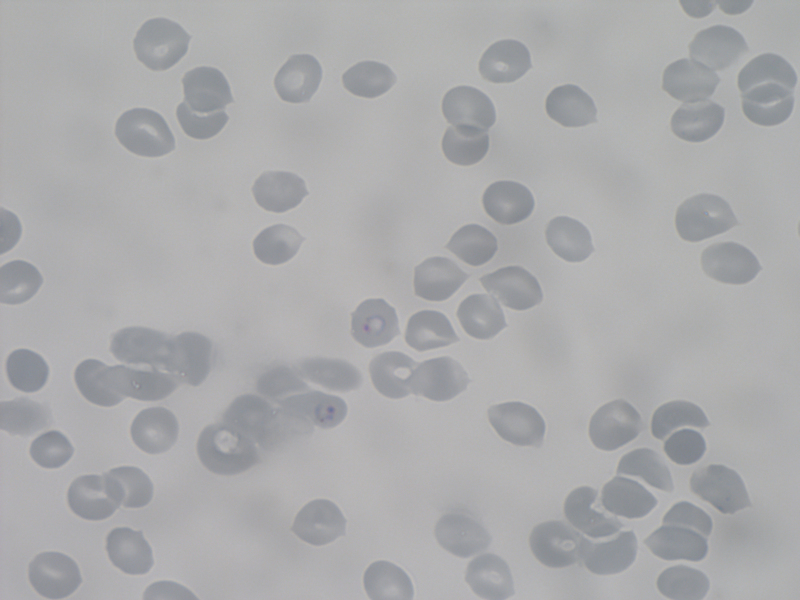
\includegraphics[width=\textwidth]{../data/natural001.jpg}
      \caption{Original image}
      \label{fig:morphology-examples-malaria-orig}
    \end{subfigure}

    \begin{subfigure}{0.25\textwidth}
      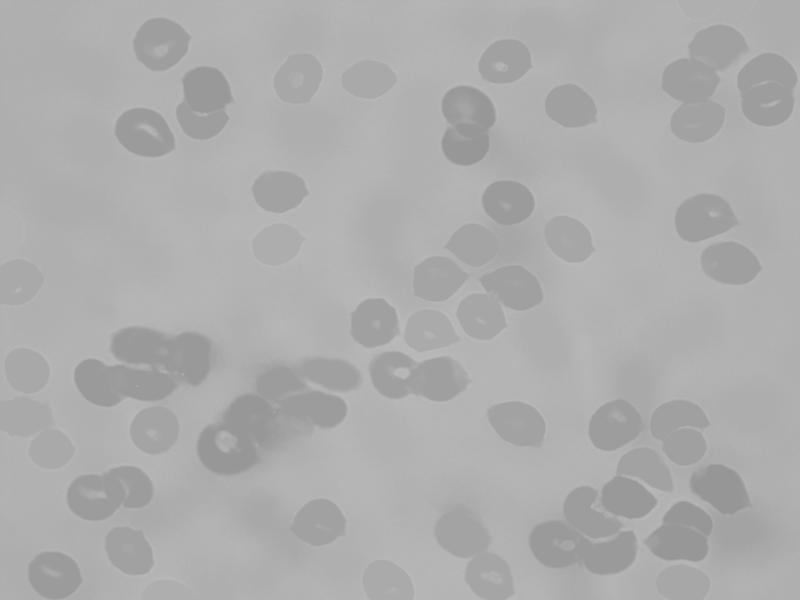
\includegraphics[width=\textwidth]{images/area-closing-1500.jpg}
      \caption{$\lambda = 1500$}
      \label{fig:morphology-examples-malaria-1500}
    \end{subfigure}

    \begin{subfigure}{0.25\textwidth}
      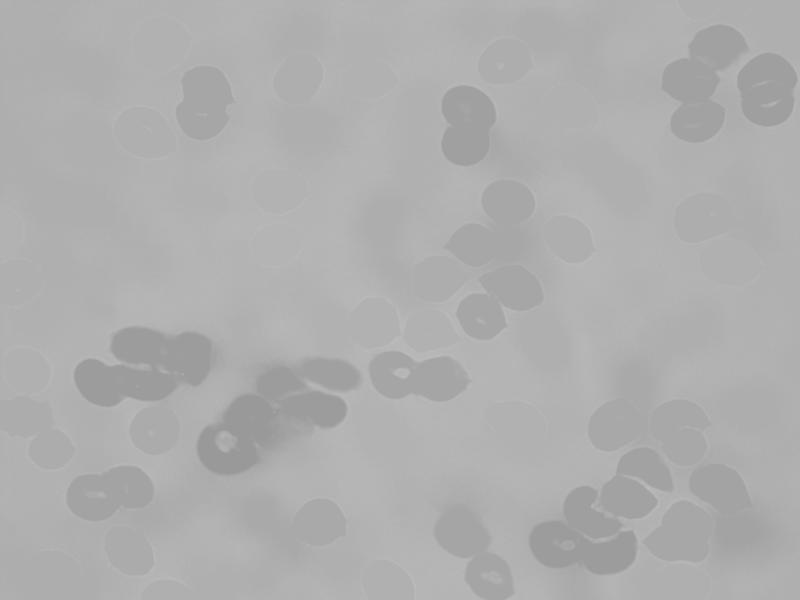
\includegraphics[width=\textwidth]{images/area-closing-3000.jpg}
      \caption{$\lambda = 3000$}
      \label{fig:morphology-examples-malaria-3000}
    \end{subfigure}

    \begin{subfigure}{0.25\textwidth}
      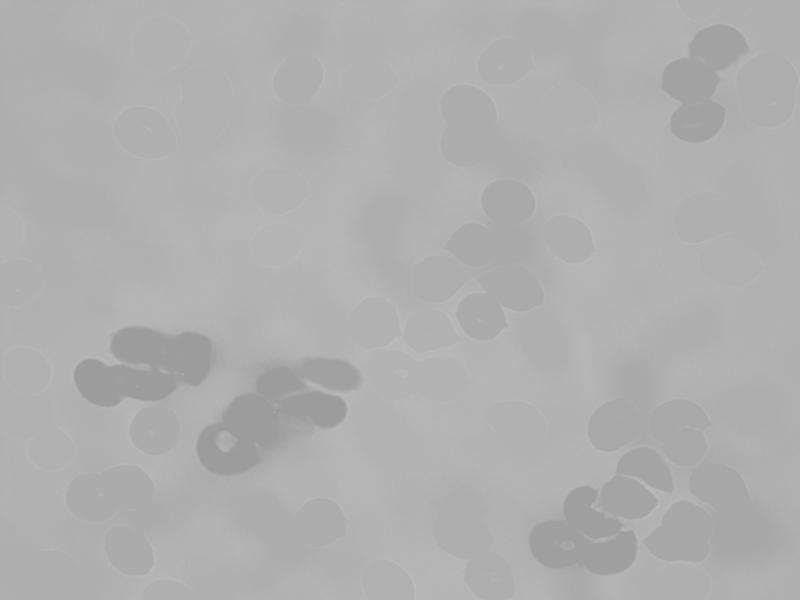
\includegraphics[width=\textwidth]{images/area-closing-4500.jpg}
      \caption{$\lambda = 4500$}
      \label{fig:morphology-examples-malaria-4500}
    \end{subfigure}

  } % makebox

  \caption[Area closing (dual to area opening) for increasing values of
  $\lambda$.]{Area closing (dual to area opening) for increasing values of
    $\lambda$ on an image of red blood cells infected with Malaria ($800 \times
    600$ pixels). The larger $\lambda$ becomes, the more blood cells are
    filtered from the image.}
  \label{fig:morphology-examples-malaria}
\end{figure}

\section{Algorithms}
\label{sec:morphology-algorithm}

There exist three well studied algorithms for computing morphological area
opening. Vincent \cite{Vincent1994Morphological} originally described an
algorithm based on gray-scale reconstruction, that requires multiple scans of
the input image using priority queues.

A faster algorithm based on Max-Trees was proposed by
\citet{Salembier1998Antiextensive}. Max-Trees are rooted trees where each node
represents a connected, flat level component. Regional maxima are represented by
the leaves of the tree. Filtering is then only a matter of removing all nodes of
size less than $\lambda$. It is easily generalized for a wide range of
morphological filters, such as morphological thinnings
\cite{Breen1996Attribute}. \citet{Wilkinson2008Concurrent} developed a parallel
version of this algorithm. They split the input image in $n \geq t$ sub-images,
where $t$ is the number of available hardware threads. For each sub-image, a
Max-Tree is computed in parallel. In a subsequent, sequential routine, the
independently computed trees are merged and, finally, filtered.

\citet{Meijster2002Comparison} proposed a region growing algorithm to compute
morphological area openings based on Tarjan's union-find data structure
\cite{Tarjan1983Data}. They extended their algorithm to compute the size
distribution of elements on an image, called area granulometry
\cite{Meijster2001Fast}. The parallel algorithms developed in this thesis extend
this union-find based algorithm. The remainder of this section contains a
detailed description of the algorithm by \citet{Meijster2002Comparison}.

A pixel $i$ at the coordinates $(x, y)$ is represented as single integer value,
computed by $i = w \cdot y + x$ where $w$ is the width of the input image
\cite{Meijster2002Comparison}. Connected components are represented by a
disjoint-tree structure, where the root of each tree is represented by the last
visited pixel. An input image is represented using two arrays:

\begin{itemize}
\item \inlinecode{value}, which stores an integer representation of the
  gray-scale value of each pixel. During the main loop, this array is read only.

\item \inlinecode{parent}, which represents the index of the parent pixel in the
  union-find data structure if \inlinecode{parent[i]} $\geq 0$, or the size of
  the tree of which \inlinecode{i} is the root, if \inlinecode{parent[i]} $< 0$.
\end{itemize}

\begin{figure}
  \centering
  \lstinputlisting[widthgobble=1*0,linerange={union0-union1}]{../parallel-morphology/src/dk/itu/parallel/morphology/unionfind/SequentialUnionFind.java}
  \caption{The \inlinecode{union} function for conditional region growing.}
  \label{fig:morphology-algorithm-union}
\end{figure}

\begin{figure}
  \centering
  \lstinputlisting[widthgobble=1*0,linerange={uniteNeighbors0-uniteNeighbors1}]{../parallel-morphology/src/dk/itu/parallel/morphology/filter/base/Filter.java}
  \caption{The \inlinecode{uniteNeighbors} function that calls \inlinecode{union}.}
  \label{fig:morphology-algorithm-uniteNeighbors}
\end{figure}

For simplicity, both arrays are also accessible through equally named
functions. Using negative integers to represent tree size instead of parent
index, allows us to minimize memory usage \cite{Meijster2002Comparison}. We are
furthermore given the following functions:

\begin{itemize}
\item \inlinecode{union(n, c, lambda)} unites the trees containing the pixels at
  \inlinecode{n} and \inlinecode{c} for a given size parameter
  \inlinecode{lambda} (see figure~\ref{fig:morphology-algorithm-union})
  \cite{Meijster2002Comparison}.

\item \inlinecode{find(x)} returns the root index of the tree containing the
  pixel at \inlinecode{x} and compresses the path between \inlinecode{x} and the
  root \cite{Tarjan1983Data, Meijster2002Comparison}.

\item \inlinecode{neighbors(x)} returns all indices of the pixels adjacent to
  \inlinecode{x}, assuming 8-connectivity.

\item \inlinecode{uniteNeighbors(x, lambda)} unites the pixel at \inlinecode{x}
  with all its valid neighbors.
\end{itemize}

To compute area opening, we must first identify regional maxima on the image
\cite{Vincent1994Morphological}. The algorithm by \citet{Meijster2002Comparison}
does this by sorting image pixels by gray-scale value. The so sorted pixel
indices are stored in an additional array \inlinecode{sorted}. Sorting can be
performed in linear time using counting-sort \cite{Meijster2002Comparison}.

The next step is to let connected components of pixels grow conditionally, if,
after the definition of area opening, neighboring connected components belong to
the same connected component. The function \inlinecode{uniteNeighbors(c, lambda)}
unites a pixel with all its valid neighbors and is shown in detail in
figure~\ref{fig:morphology-algorithm-uniteNeighbors}.

If \inlinecode{c} is at level with \inlinecode{n}, the pixel pair is valid. This
is essentially flat component labeling \cite{Meijster2002Comparison}. Moreover,
a pixel is allowed to join a set ``upwards'' in gray-level hierarchy, so to
unite with a pixel of higher gray-value: this is the first part of growing
connected components. The gray-level sorted pixels are iterated in decreasing
gray-value order. This is the main loop of union-find based area opening
\cite{Meijster2002Comparison}:

\lstinputlisting[linerange={filter0-filter1},frame=L]{../parallel-morphology/src/dk/itu/parallel/morphology/filter/Sequential.java}

However, \inlinecode{union} does not unite disjoint trees
unconditionally. Instead, it allows connected components only to be united, if
either the root of \inlinecode{n} is at level with \inlinecode{c}, or, if the
area of the connected component containing \inlinecode{n}, is less than
\inlinecode{lambda}. If none of these conditions are fulfilled, \inlinecode{c}
is deactivated: its size is simply set to \inlinecode{lambda} and no component
may exceed \inlinecode{lambda}, unless it is a level-component (i.e. all pixels
of the component are at the same gray-level) \cite{Meijster2002Comparison}. If
the trees are united, the last visited pixel \inlinecode{c} becomes the new
root. Thereby, the darkest pixel of the connected component is always the root
of the tree. Building paths in this fashion directly contradicts the idea of
ranking and swapping trees, in order to maintain short paths
\cite{Tarjan1983Data}. \citet{Meijster2002Comparison} leave this contradiction
uncommented.

This algorithm a simplified version of the one given by
\citet{Meijster2002Comparison}. Their original algorithm performs on-the-fly
initialization of the disjoint set structure, which is possible because, in a
sequential program, counting sort is stable w.r.t. the prior order of
elements. This implies that it is enough to find the root of \inlinecode{n}
during \inlinecode{union}, as \inlinecode{c} has not yet been initialized as a
singleton. Every pixel's singleton is initialized when
\inlinecode{uniteNeighbors} is called on it. The original condition (compared to
figure~\ref{fig:morphology-algorithm-uniteNeighbors}), to determine whether a
pixel should be united with its neighbors, is \cite{Meijster2002Comparison}:

\begin{lstlisting}[style=inline]
  value(c) <= value(n) || (value(c) == value(n) && n < c)
\end{lstlisting}

This structure gives the linear code advantages, which are hard to achieve in
parallel algorithms. For the remainder of this thesis, I will only consider the
simplified version of the algorithm, so that the order of level pixels is
neglected. The detailed implementation of the simplified \inlinecode{union}
algorithm is depicted in figure~\ref{fig:morphology-algorithm-union}.

Always making the last visited, and thereby darkest, pixel root of its set
enables us to use a simple resolving step, that finalizes the algorithm. The
list of sorted pixels is iterated in reverse order and each pixel is assigned
the gray-scale value of its root. Thereby, we filter regional maxima from the
image \cite{Meijster2002Comparison}:

\begin{lstlisting}[frame=L]
    // Resolve gray-values.
    for (final int s : sorted) {
      if (parent(s) > 0) // Only update child-nodes.
        image().pixel[s] = value(find(s));
    }
\end{lstlisting}

This final step will not be part of further discussion, as it can easily be
parallelized. We are mainly interested in building the correct union-find
structure to represent connected components.

%%% Local Variables:
%%% mode: latex
%%% TeX-master: "main"
%%% End:


\chapter{Shared Union-Find Data Structures}
\label{chpt:union-find}

This chapter describes two different algorithms for a shared union-find
\cite{Tarjan1983Data} data structure. The first one is the wait-free union-find
algorithm by \citet{Anderson1994Waitfree}. The other one relies
on fine-grained locking per disjoint tree \cite{Berman2010Multicore}.

The following sections contain many different figures, that convey variants of
parallel union-find. In order to explain the algorithms thoroughly, I believe
that it is easiest for the reader to look at code examples. This is especially
true, because the many variants of the union-find algorithm are very similar and
the differences are very subtle, if explained in plain English. I deliberately
omit introducing the original union-find by \citet{Tarjan1983Data} in favor of
focusing on the concurrent algorithms.

\section{A Wait-Free Implementation}
\label{sec:union-find-wf}

As described in section \ref{sec:introduction-concurrency}, wait-free concurrent
algorithms have a number of desirable properties, compared to blocking
algorithms. Therefore, \citet{Anderson1994Waitfree} developed a wait-free
union-find algorithm, based on the \emph{CAS} primitive. Their implementation
uses ranking heuristics to balance trees, in order to maintain short chains
between leafs and roots.

The wait-free union-find algorithm represents nodes in an array of records,
called \inlinecode{record} and again accessible through a function of the same
name. Each \inlinecode{Record} contains an integer representation of the rank
of a tree and an (atomic) integer pointing to the index of the record's parent
in the array. The implementation of \inlinecode{Record} is shown in
figure~\ref{fig:union-find-wf-union-record}.

\begin{figure}
  \centering
  \lstinputlisting[linerange={record0-record1}]{../parallel-union-find/src/dk/itu/parallel/unionfind/WaitFree.java}
  \caption[The \inlinecode{Record} class, as used in wait-free union-find.]{The
    \inlinecode{Record} class, as used in wait-free union-find. Maintaining the
    rank and the pointer to the node's parent in this object allows an atomic
    update of both variables using \emph{CAS}.}
  \label{fig:union-find-wf-union-record}
\end{figure}

The parent pointer initially points to the index of the record itself, to
indicate that it is a root. It is here implemented as an atomic reference, to
make implementing a wait-free path-compressing \inlinecode{find} easy. If
\inlinecode{find} was not to compress paths, it could simply traverse up to the
root. This would be wait-free already, as \inlinecode{find} does not guarantee
anything but to return a node that was root at some point in time
\cite{Anderson1994Waitfree}. To compress paths in a wait-free manner,
\citet{Anderson1994Waitfree} implement their find using path-halving:

\lstinputlisting[style=inline, linerange={find0-find1}]{../parallel-union-find/src/dk/itu/parallel/unionfind/WaitFree.java}

The parent pointer of each visited node is set to the node's grandparent, if no
other thread modified the parent pointer in the meantime. If another thread
interfered, the failed \emph{CAS} is simply ignored and traversal continues.

Uniting two disjoint trees is a matter of updating the parent pointer of a node,
as well as its rank. To perform this update atomically,
\citet{Anderson1994Waitfree} use the \inlinecode{Record} object associated with
this node. The record of the node, which will be updated, is atomically replaced
by a record pointing to the new record and maintaining a new rank. This update
is performed by the auxiliary function \inlinecode{updateRoot}. It terminates
early, if another thread modified the soon-to-be child node at
\inlinecode{x}. Otherwise, it simply returns to the caller, whether the update
has been successful:

\lstinputlisting[style=inline, linerange={updateroot0-updateroot1}]{../parallel-union-find/src/dk/itu/parallel/unionfind/WaitFree.java}

While this would already be enough to implement a wait-free \inlinecode{union},
\citet{Anderson1994Waitfree} acknowledge, that this can result in long chains,
if multiple threads unite trees, without the rank of the root being incremented
successfully. To counter this, they add a call to \inlinecode{setRoot}, which
performs a \inlinecode{find}-like traversal and compression. Finally,
\inlinecode{setRoot} tries to update the rank of the root by one atomically,
using \inlinecode{updateRoot}:

\lstinputlisting[style=inline, linerange={setroot0-setroot1}]{../parallel-union-find/src/dk/itu/parallel/unionfind/WaitFree.java}

The \inlinecode{union} function, in its entire form, is depicted in figure
\ref{fig:union-find-wf-union}.

\begin{figure}
  \lstinputlisting[linerange={union0-union1,union2-union3,union4-union5}]{../parallel-union-find/src/dk/itu/parallel/unionfind/WaitFree.java}
  \caption[Wait-free implementation of \inlinecode{union}.]{Wait-free
    implementation of \inlinecode{union}. \citet{Anderson1994Waitfree}
    acknowledge, that this implementation of concurrent \inlinecode{union} can
    result in long chains in the disjoint tree structure.}
  \label{fig:union-find-wf-union}
\end{figure}

\subsection{Adaption to Area Opening}
\label{sec:union-find-wf-adaption}

A major flaw of \citeauthor{Anderson1994Waitfree}'s wait-free union-find
algorithm is the spuriously occurring failure of updating ranks, as well as the
temporary inconsistencies between node updates \cite{Anderson1994Waitfree,
  Berman2010Multicore}. Updating the size of a root node, together with updating
references to it, is key to label connected components correctly. Otherwise,
another thread could grow a component, while another is in-between updating the
root pointer and updating the new root's size, which are independent from each
other. This can result in uniting pixel sets based on wrong priorities. Using
\inlinecode{Record} as a container to update rank and parent pointer atomically,
works only for updating both values on the same node and does therefore not
provide a solution to the problem.

This is a manifestation of the missing composition capabilities of
synchronization primitives, as already mentioned in section
\ref{sec:introduction-cas}. \citet{Herlihy2008Art} give a proof, that there is
no wait-free implementation to assign values to multiple, independent fields
(i.e. an $(m,n)$-assignment) consistently.

This means that the wait-free union-find algorithm cannot be directly applied to
our problem.

\subsection{STM Variant}
\label{sec:union-find-wf-stm}

To update two independent nodes atomically when computing area opening, we can
resort to an \emph{STM} version of \citeauthor{Anderson1994Waitfree}'s
algorithm. The \inlinecode{find} routine stays entirely wait-free and still
performs path compression by path-halving, as shown in
figure~\ref{fig:union-find-wf-stm-find}. It is now mandatory to avoid compressing the path
to a negative parent pointer, as that would result in removing a sub-tree from
its root.

\begin{figure}
  \centering
  \lstinputlisting[linerange={find0-find1}]{../parallel-morphology/src/dk/itu/parallel/morphology/unionfind/Transactional.java}
  \caption[Wait-free \inlinecode{find} for area opening.]{Wait-free
    \inlinecode{find} for area opening. \emph{multiverse}'s
    \inlinecode{atomicWeakGet} corresponds to \inlinecode{get} on Java's atomic
    types; \inlinecode{atomicCompareAndSet} corresponds to
    \inlinecode{compareAndSet}. As soon as the \inlinecode{parent} value of a
    node is equal or below zero, it will not be set to below zero again.}
  \label{fig:union-find-wf-stm-find}
\end{figure}

The concept of records is not required any longer. Also, ranking and the
according rank updates are removed, in order to model the correct relation of
pixels to each other \cite{Meijster2002Comparison}. This implies also the
removal of \inlinecode{updateRoot} and \inlinecode{setRoot}.

The wait-free \inlinecode{union}'s while-pattern is still required by the
algorithm, if we use negative values to model component size, while compressing
the paths using a wait-free \inlinecode{find}. Otherwise, we can run into
complications when checking, whether the negated parent value (i.e. the size) is
less than \inlinecode{lambda} (see figure \ref{fig:union-find-wf-stm-union}).

\begin{figure}
  \centering
  \lstinputlisting[linerange={union0-union1,union2-union3,union4-union5}]{../parallel-morphology/src/dk/itu/parallel/morphology/unionfind/Transactional.java}
  \caption[STM \inlinecode{union} for area opening.]{STM \inlinecode{union} for
    area opening. \inlinecode{TxnVoidCallable} is a \emph{multiverse} wrapper
    class, similar to the \inlinecode{Callable} interface. Note that the
    while-loop is still required, in order to catch modifications by wait-free
    \inlinecode{find}.}
  \label{fig:union-find-wf-stm-union}
\end{figure}

Moreover, we can implement conditional deactivation of not-united root nodes. If
a to-be-deactivated root already exceeds \inlinecode{lambda}, it does not need
to be deactivated explicitly. Short-circuiting this operation saves overhead due
to unnecessary modifications by the transaction, which would otherwise come at
the considerable cost of copying and modifying the variable and then committing
the changes \cite{Herlihy2008Art}.

To compare the performance of using an explicit while-loop , I implemented a
general version of \citeauthor{Anderson1994Waitfree}'s union-find with
\emph{STM} modifications, as well as a simple \emph{STM} implementation. The
latter simply wraps the sequential \inlinecode{union} in a single transaction.

\section{An Optimistic Implementation}
\label{sec:union-find-optimistic}

\begin{figure}

  \lstinputlisting[linerange={union0-union1,union2-union3,union4-union5}]{../parallel-union-find/src/dk/itu/parallel/unionfind/Optimistic.java}

  \caption[Optimistic locking implementation of \inlinecode{union}.]{Optimistic
    locking implementation of \inlinecode{union}. The algorithm performs
    \inlinecode{find}, until it has acquired the locks for the actual roots.}
  \label{fig:union-find-optimistic-union}
\end{figure}

Typically, locks are used globally for data structures. This blocks threads from
performing changes, while another thread is modifying some part of the
data. While easier to implement, this leads to high contention, as the progress
of all threads \emph{not} holding the global lock is blocked, even if their
modifications would not collide with those of the active thread. This is not
acceptable for efficient parallel algorithms.

Another approach is optimistic, or fine-grained, locking of resources. A thread
only acquires locks for those parts of a data structure, that it wants to modify
consistently. Writing to an array at different indices is probably the best
example for a data structure, that invites such a locking scheme, as each index
of the array can get assigned a unique lock.

In his thesis, \citet{Berman2010Multicore} developed a union-find algorithm
based on optimistic locking. He claims that this approach outperforms the
wait-free union-find implementation by \citet{Anderson1994Waitfree}. In his
implementation, the disjoint sets are represented by three arrays of the same
length: one array \inlinecode{next}, that, for each node, holds a pointer to
either the parent index or to itself, if it is root. Another array
\inlinecode{rank}, that maintains the rank of each node, and finally an array
\inlinecode{lock}, that maintains a lock for each node in the disjoint set
structure \cite{Berman2010Multicore}.

To update the relation of two trees consistently, \citet{Berman2010Multicore}
uses a (not further described) function \inlinecode{lock\_roots} that locks two
trees in the forest of disjoint trees by acquiring the locks only for the
respective root nodes. Java does not provide a two-object locking
mechanism. Therefore, the Java implementation uses a simple double-lock
algorithm on the \inlinecode{lock} array, which is of type
\inlinecode{ReentrantLock[]}. This algorithm is based on a simple lock algorithm
given by \citet{Herlihy2008Art}. Unlocking both trees, in case acquiring both
locks failed, ensures that no deadlocking occurs, in case a thread only
successfully acquired one lock:

\lstinputlisting[style=inline, linerange={lock0-lock1}]{../parallel-union-find/src/dk/itu/parallel/unionfind/Optimistic.java}

\citet{Berman2010Multicore} proposes a scheme that, once it acquired the locks
for two nodes, checks that these nodes are still roots. The fine-grained locking
makes it possible for the nodes to change their state, while a thread waits to
acquire their locks. In the Java implementation, this locking scheme is
integrated into \inlinecode{union}, as shown in figure
\ref{fig:union-find-optimistic-union}.

Another notable difference to the wait-free algorithm is the path
compression. The optimistic algorithm compresses paths only after successfully
uniting two sets, while still holding the locks \cite{Berman2010Multicore}. This
makes \inlinecode{find} fully wait-free, as no locks must be acquired during
traversal. Path compression is implemented by re-assigning the parent pointer of
each node along the path to the root's index.

\subsection{Adaption to Area Opening}
\label{sec:union-find-optimistic-adaption}

For the optimistic union-find implementation, the changes for using it in area
opening are nearly negligible. Here as well, both pixel's roots must be found
prior to proceeding. Updating the size of a tree at the root node and the parent
pointer of another node, in order to make it to point to the new root, is not an
issue in a lock-based implementation. Again, ranking heuristics are removed
\cite{Meijster2002Comparison}.

\begin{figure}
  \centering
  \lstinputlisting[linerange={compress0-compress1}]{../parallel-morphology/src/dk/itu/parallel/morphology/unionfind/Optimistic.java}
  \caption[The \inlinecode{compress} function for optimistic area opening.]{The
    \inlinecode{compress} function for optimistic area opening. It is only
    executed when the thread holds the corresponding lock for the node at
    \inlinecode{root}.}
  \label{fig:union-find-optimistic-adaption-compress}

  \lstinputlisting[linerange={union0-union1,union2-union3}]{../parallel-morphology/src/dk/itu/parallel/morphology/unionfind/Optimistic.java}
  \caption[Optimistic \inlinecode{union} for area opening.]{Optimistic
    \inlinecode{union} for area opening. The paths are compressed w.r.t. success
    or failure of uniting the two sets.}
  \label{fig:union-find-optimistic-adaption-union}
\end{figure}

In order to determine whether found nodes are still roots, it is sufficient to
check, whether their \inlinecode{parent} value is below zero. As soon as a
node's \inlinecode{parent} value is equal to or greater than zero, it will not
be re-set to below zero, since this union-find structure does not support
deletion. The same goes for the wait-free implementation of \inlinecode{find}.

Another modification is the compression of paths (see
figure~\ref{fig:union-find-optimistic-adaption-compress}), which depends on the
success or failure of conditional union. If the trees have been united, both
trees are compressed to the same root. Otherwise, their respective original
roots are used as compression targets. The complete algorithm for optimistic
\inlinecode{union}, adapted to area opening, is shown in
figure~\ref{fig:union-find-optimistic-adaption-union}.

%%% Local Variables:
%%% mode: latex
%%% TeX-master: "main"
%%% End:


\chapter{Parallel Area Opening}
\label{chpt:area-opening}

In this section, I will describe five algorithms that compute the area opening
for a given input image and a minimum area $\lambda$, in parallel. All
algorithms are implemented, so that they can use either variant of shared
union-find as presented in chapter \ref{chpt:union-find}.

The designs of the parallel area opening algorithms vary to different
degrees. The first important notion is that of work items. For images, those are
typically either pixels, pixel-lines or multi-line sub-images. Furthermore,
there are essentially three types of filtering algorithms:

\begin{description}
\item[No sorting] Instead of sorting, the pixel array is scanned repeatedly.

\item[Thread-local sorting] Subsets of the pixel array are sorted
  thread-locally.

\item[Shared sorting] Pixels are sorted in a lock-free fashion and sorting is a
  joint effort of all threads.

\end{description}

There is one important property, that may not be violated by any algorithm:
pixels must be scanned in decreasing gray-scale order, in order to guarantee,
that regional maxima are found implicitly \cite{Meijster2002Comparison}. We will
get back to the importance of this property in chapter \ref{chpt:correctness}.

In the following sections, we will see implementation details for each of these
algorithms. The algorithms can handle any number of gray-scale values. The
resolving step, that updates the gray-scale values of each pixel, according to
its position in the tree, is omitted entirely: this is a linear time operation
\cite{Meijster2002Comparison} and can easily be parallelized.

For the remainder of this chapter, let $k$ denote the number of possible
gray-values per pixel, and $n$ the number of pixels in a gray-scale image
$I$. Moreover, let $x_I$ and $y_I$ denote the dimensions of an image $I$ in $x$-
and $y$-direction, so that $x_I y_I = n$. To simplify the analysis of the
algorithms, let us assume that \inlinecode{uniteNeighbors} amortizes to $O(n)$
for an image $I$ of size $n$. We will only use formal run-time complexity to
underline, how differently the parallel algorithms behave, even though they
share the same formal complexity.

\section{Non-Sorting Variants}
\label{sec:area-opening-no-sorting}

A key idea of the algorithm presented by \citet{Meijster2002Comparison}, is to
sort pixels in linear time by gray-value. Originally, Vincent proposed an
algorithm, that scans the image repeatedly \cite{Vincent1994Morphological}. In
this section, we will take a look at algorithms that neglect the possibility of
linear-time sorting of pixels and instead re-scan the image, until all pixels
have been filtered. The main purpose is didactic: without sorting, the
algorithms are easier to implement and we can focus on key ideas. In
section~\ref{sec:area-opening-local-sorting}, we will see algorithms that extend
the ones presented here, by sorting the input. Nevertheless, algorithms from
this section will be included in the performance evaluation in
chapter~\ref{chpt:experiments}.

\subsection{Sub-Image Filtering}
\label{sec:area-opening-no-sorting-sub-image}
\begin{figure}
  \centering

  \lstinputlisting[widthgobble=2*1, linerange={filter0-filter1}]{../parallel-morphology/src/dk/itu/parallel/morphology/filter/Split.java}

  \caption[Simple sub-image filtering algorithm.]{Simple sub-image filtering
    algorithm. The interval of pixels assigned to a thread is denoted as the
    integers \inlinecode{lower} and \inlinecode{upper}. Threads synchronize on
    gray-level decrease.}
  \label{fig:area-opening-no-sorting-sub-image}
\end{figure}

A typical pattern to parallelize image analysis algorithms, is to simply split
up the image in as many sub-images as there are hardware threads available. This
requires, that the operation on each pixel is independent. This approach works
well for image convolutions, such as the Sobel filter
\cite{Szeliski2011Computer}.

According to these requirements, conditional region-growing, as performed during
area opening, is not parallelizable by splitting the image: correct growing must
be ensured across sub-image borders. Using a shared and re-entrant data
structure, however, like our concurrent union-find variants, circumvents this
requirement of independence. While each operation can be performed
independently, the result of each union operation is shared across threads
implicitly through side-effects.

Following this, we can implement a simple area opening algorithm on
sub-images. Each hardware thread is assigned an upper and a lower index on the
pixel array of the image and, for each gray-scale level, iterates repeatedly
over all indices, from the lower to the exclusive upper bound, uniting all valid
pixels for the current gray-scale level. All threads are synchronized on the
current gray-level, which is maintained locally by each thread. Synchronization
is performed through a barrier: on reaching the barrier, a thread may not
proceed, until all other threads also reach it.

If executed on only a single hardware-thread, the complexity of non-sorting
sub-image area-opening is $O(kn)$. This algorithm is detailed in figure
\ref{fig:area-opening-no-sorting-sub-image}.

\subsection{Pixel Queues}
\label{sec:area-opening-no-sorting-pixel-queues}

\begin{figure}
  \centering

  \lstinputlisting[widthgobble=2*1, linerange={filter0-filter1}]{../parallel-morphology/src/dk/itu/parallel/morphology/filter/QueuePixels.java}

  \caption[Pixel queue filtering algorithm.]{Pixel queue filtering
    algorithm. Pixels are re-added to the \inlinecode{lower} queue, if their
    gray-level is less than the current level.}
  \label{fig:area-opening-no-sorting-pixel-queues}
\end{figure}

The naive sub-image filtering algorithm, as shown in
section~\ref{sec:area-opening-no-sorting-sub-image}, always runs in $O(kn)$: all
pixels need to be scanned again for each gray-level of the image. If we want to
take advantage of the fact, that each pixel only needs to be filtered explicitly
once, we need a way to remove already filtered pixels from the work-list.

A way to represent not yet filtered images is a concurrent queue data structure,
for instance a \citet{Michael1996Simple} queue (see also
section~\ref{sec:introduction-msq}) or a lock-free, bounded array queue (see
implementation details of this data structure in
appendix~\ref{sec:bounded-array-queue}). At initialization time, all pixels are
added to the queue. This can be done in parallel by all threads. Then, each
thread removes the next pixel from the tip of the queue and either filters the
pixel, if it is at the current gray-level, or adds it to the end of the queue
again.

This approach has two issues: first, we would need to keep track of how many
pixels we already have filtered and how many pixels we still expect to be in the
queue, in order to decrease the current gray-level correctly. Secondly (and
actually less importantly), we would encounter many conflicts during
concurrently removing and adding pixels.

To simplify the approach, we can instead use two queues, wrapped in a container
class \inlinecode{Queues} (see appendix~\ref{sec:area-opening-queues} for
details). It maintains one active, or upper, queue, that contains all pixel
indices, that still need to be filtered for the current level, and one inactive,
or lower, queue, to which all pixels that have not been filtered yet, are
added. Now, the current gray-level can safely be decreased when the active queue
is empty. The auxiliary function \inlinecode{swapAndDecrement} decrements the
current gray-level and swaps active and inactive queues atomically. The
implementation of \inlinecode{swapAndDecrement} is detailed in
appendix~\ref{sec:area-opening-queues}.

Analytically, this is still a linear-time operation. Assuming, that both adding
and removing a pixel from a queue happens in constant time, the worst-case has a
complexity of $O(n + kn) = O(kn)$. The algorithm is detailed in
figure~\ref{fig:area-opening-no-sorting-pixel-queues}.

\section{Thread-local Sorting Variants}
\label{sec:area-opening-local-sorting}

In this section, we will consider algorithms, that sort pixels in a thread-local
manner. That means, that each thread executes a sequential sorting algorithm on
some portion of pixels. The algorithms in this section extend the algorithms
presented in section~\ref{sec:area-opening-no-sorting}.

\subsection{Sub-Image Filtering}
\label{sec:area-opening-local-sorting-sub-image}

\begin{figure}
  \centering

  \lstinputlisting[widthgobble=2*1, linerange={filter0-filter1}]{../parallel-morphology/src/dk/itu/parallel/morphology/filter/SplitCounting.java}

  \caption[Sub-image filtering algorithm with thread-local sorting.]{Sub-image
    filtering algorithm with thread-local sorting. The sub-images are sorted
    prior to filtering in order to avoid multiple scans of the image.}
  \label{fig:area-opening-local-sorting-sub-image}
\end{figure}

The naive image splitting algorithm
(section~\ref{sec:area-opening-no-sorting-sub-image}), does not make any use of
the pixel properties, that allow linear-time sorting. To improve the algorithm's
run-time complexity, we now first let each thread sort the pixels in its
assigned interval and thereby remove the need for multiple scans of the
image. Threads still synchronize on gray-level decrease. This results in a
run-time complexity of $O(k + n + n) = O(k + n)$.

In the Java implementation
(figure~\ref{fig:area-opening-local-sorting-sub-image}), I use counting sort, as
suggested by \citet{Meijster2002Comparison}. The algorithm terminates, if the
current gray-level is below zero, i.e. all gray-levels have been
filtered. Otherwise, we need to check, whether the current pixel's value is
equal to the current gray-level and only filter it, if this is the case. If all
pixels in this interval have been filtered, we assign -1 to the current pixel
pointer \inlinecode{c}. If \inlinecode{c < 0}, we can directly jump to
decrementing the thread-local level pointer and to synchronizing threads.

\subsection{Line Queues}
\label{sec:area-opening-local-sorting-queues}

\begin{figure}
  \centering

  \lstinputlisting[widthgobble=2*1, linerange={filter0-filter1}]{../parallel-morphology/src/dk/itu/parallel/morphology/filter/QueueLines.java}

  \caption[Line queue filter algorithm with thread-local per-line sorting.]{Line
    queue filter algorithm with thread-local per-line sorting. The pixels of
    each line are sorted via counting sort. Lines are shared across threads, in
    order to avoid starvation. The \inlinecode{Line} interface provides
    transparent access to the sorted pixels and maintains an internal pointer to
    the current pixel.}
  \label{fig:area-opening-local-sorting-queues}
\end{figure}

The queue-based approach from
section~\ref{sec:area-opening-no-sorting-pixel-queues} to parallel area opening
can easily be extended to the next greater unit of work-items in images. A class
\inlinecode{Line} represents a line, containing an array of pixel indices (see
appendix~\ref{sec:pixel-line}). It maintains an internal pointer to the current
pixel index. The pointer can be moved transparently by a call to
\inlinecode{advance}, which returns a Boolean indicating the success of the
operation. It will fail, if there is no work left (i.e. all pixels have been
filtered), which can also be queried directly using \inlinecode{workLeft} (see
the full implementation in appendix~\ref{sec:pixel-line}).

All threads join in the initialization phase, where each processes a line at a
time thread-locally. Each line is sorted separately, using again counting
sort. After the initialization phase, the double queue principle, as shown in
section~\ref{sec:area-opening-no-sorting-pixel-queues}, is used. The Java
implementation is displayed in
figure~\ref{fig:area-opening-local-sorting-queues}.

The advantage of this algorithm is two-fold. First, removing the requirement for
re-scanning the image, or parts of it, is removed entirely. All work-items,
pixels and lines, are removed from the queues as soon as they have been
filtered. Secondly, this approach avoids a problem that can hurt the performance
of sub-image filtering badly, causing extreme starvation. Consider the case of a
gray-scale gradient in the image's $y$-direction. Using a sub-image filtering
approach, this case essentially forces the threads to work in sequence, waiting
idly for the one thread that is lucky to be assigned the sub-image, which holds
all pixels of the current gray-level. This is not longer possible with the
line-queues algorithm, as threads are not assigned a fixed portion of work, but
share all data to support progress actively.

The worst-case run-time complexity of the line-queues algorithm bases on the
initialization-step, which is (sequentially) of $O(y_I(k + x_I)) = O(y_Ik +
n)$. An additional cost is, of course, the union of pixels with their neighbors
and the re-adding of each line of $O(y_I + n)$, so overall we get $O(y_Ik + y_I
+ 2n) = O(y_Ik + n)$.

\section{Shared Sorting Variants}
\label{sec:area-opening-shared-sorting}

\begin{figure}
  \centering

  \lstinputlisting[widthgobble=2*1, linerange={filter0-filter1}]{../parallel-morphology/src/dk/itu/parallel/morphology/filter/BlockGrayLevel.java}

  \caption[Per-level blocking filter algorithm with shared sorting.]{Per-level
    blocking filter algorithm with shared sorting. The threads are again
    synchronized on gray-level decrease.}
  \label{fig:area-opening-shared-sorting}
\end{figure}

The last variant is to share the work of sorting the pixels of the image between
all threads. Each thread iterates, in parallel, over the shared array of sorted
pixels and performs \inlinecode{uniteNeighbors}, synchronizing again on
gray-scale level decrease.

There are two linear-time sorting algorithms that can be parallelized
easily. The first one is the already mentioned counting-sort. To obtain a fully
parallel variant, we cannot rely on partitioning the input data. Instead, the
implementation here uses atomic integers and barriers to sort in parallel. One
side-effect is, that the target array cannot be re-used, causing an increase of
memory usage by $O(n)$. Also, the parallel sorting algorithm is not wait-free,
since we need to synchronize between counting and insertion steps.

The second algorithm is bucket sorting by maintaining an array of re-entrant
queues. The array is of length $k$, with each index representing the subset of
pixels at the indexes gray-scale level. To not cause a memory usage of $O(kn)$
($k$ levels with possibly $n$ pixels each), it is mandatory to use an unbounded
data structure, in order to maintain those subsets. I therefore chose to use
Michael-Scott queues in order to keep memory usage low.

Both algorithms are implemented in a data structure, that implements the
\inlinecode{LinearPixelSort} interface. A thread can seamlessly start sorting by
calling \inlinecode{sort} on a sub-type of \inlinecode{LinearPixelSort}, since
the lock-free structure of both algorithms requires no knowledge of the number
of threads participating in parallel sorting. Calling \inlinecode{next}, with a
gray-scale level as argument, returns the next pixel at the given level, or
\inlinecode{null}, if there are no pixels left at this level.

Shared sorting is followed by gray-level wise filtering of pixels. The
\inlinecode{level} variable is thread-local, to avoid additional
contention. Each thread then retrieves the next pixel from the current level's
queue. If retrieval was successful, i.e. the queue at the current level is not
yet empty, the pixel is united with its valid neighbors. If not, the local level
is decreased and the threads synchronize at the barrier. The full Java
implementation of the filtering part of the algorithm is given in figure
\ref{fig:area-opening-shared-sorting}. If executed sequentially, its run-time
complexity is $O(k + n + n) = O(k + n)$

%%% Local Variables:
%%% mode: latex
%%% TeX-master: "main"
%%% End:


\chapter{Correctness}
\label{chpt:correctness}

This chapter is devoted to the correctness of the algorithms presented in
chapter~\ref{chpt:area-opening}. An inherent problem of parallel and concurrent
programs is the non-determinism of interleavings between independent
threads. Because of this, standard unit-testing of parallel code, as done with
sequential code, is not enough to ensure the absence of errors.

Instead, there exist a number of formal methods to verify parallel programs. One
of the first formal frameworks to reason about correctness in concurrent
programs developed, was \emph{Communicating Sequential Programs} (CSP)
\cite{Hoare1978Communicating}. CSP allows manual reasoning and proving of
programs, but there also exist digital implementations \cite{Roscoe1997Theory}.

Another, more practical approach is model checking \cite{Visser2003Model}. The
advantage of model checking is that it can easily be fully automated. However,
model checking suffers from analyzing huge state-spaces. In this chapter, I will
focus on showing the absence of errors in the parallel area opening algorithms
through model checking by explicit state enumeration using \emph{Java
  Pathfinder} \cite{Visser2003Model}. Additionally, I will briefly touch upon
the possibilities of unit-testing parallel area opening.

\section{Experimental Correctness Verification}
\label{sec:correctness-experimental}

In contemporary software engineering, unit-testing is an often used tool to
assure that independent parts of a program behave correctly. Input values must
be provided manually, which means that testing is basically experimental
correctness verification and by no means exhaustive -- this is true for both
sequential and concurrent programs. Nevertheless, it is a good starting point in
practice. Especially parallel algorithms can, as a first step, be tested on a
single thread to assure conceptual correctness.

Due to the already pointed out non-determinism of thread interleavings -- caused
either by true hardware parallelism or by the intransparent heuristics of a
thread scheduler -- testing of truly parallel algorithms is practically
impossible. Errors might seem to occur randomly, or so spuriously that they are
not found during testing \cite{Goetz2006Java}. To increase the chance to hit
erroneous execution paths, tests can of course be repeated automatically with a
huge variety of input data. Still, this is not exhaustive. Thread scheduling is
non-deterministic, but not entirely random. Executing a concurrent program
multiple times does not guarantee to execute different thread
interleavings. Therefore, more elaborate methods are required, in order to
verify the correctness of parallel programs.

For development purposes, I implemented an experimental black-box testing suite,
which asserts a single post-condition for the parallel algorithms. Recall from
section~\ref{sec:morphology-area-opening} that $\gamma^a_{\lambda}$ denotes area
opening and $f$ a projection from a subset of $\mathbb{R}^2$ into
$\mathbb{R}^*$. Let, moreover, $\rho^a_{\lambda}$ denote any parallel variant of
area opening. We assert that:

\begin{equation}
  \label{eq:correctness-experimental-post}
  \gamma^a_{\lambda}(f) = \rho^a_{\lambda}(f)
\end{equation}

Again, due to the non-determinism of thread scheduling, this assertion might
only fail occasionally for incorrect programs.

\section{Java Pathfinder}
\label{sec:correctness-jpf}

Java Pathfinder (JPF) is an explicit state enumerator and model checker
\cite{Visser2003Model}. JPF has been used to verify concurrent real-life
\emph{NASA} programs and has discovered serious bugs \cite{Visser2004Test}. The
model checker uses search heuristics to execute all relevant states of a
program. It reports erroneous operations, such as accessing fields on
\inlinecode{null} objects or division by zero. Additionally, programs can be
annotated with pre- and post-conditions, as well as class invariants, to model
more complex correctness properties.

JPF can be seen as a drop-in JVM replacement and has been especially designed to
uncover concurrency related bugs \cite{Visser2003Model}. Any Java program can be
run directly in JPF, with the exception of programs that use native code. JPF
aware programs (those that are annotated with properties) benefit most from
model checking and, theoretically, no code-changes are required when moving the
model checked target code to a production system running a typical JVM.

\subsection{Symbolic Execution}
\label{sec:correctness-jpf-symbolic}

Symbolic execution is a method of model checking that computes values of
variables, in order to execute each path of the program once
\cite{Khurshid2003Generalized}. Thereby, it is not necessary to execute the
system under test (SUT) with many different input variables to trigger each path
once, possibly re-taking already executed and checked program paths. Symbolic
variables are assigned as needed, to trigger all possible program paths. This is
trivial for data types like Boolean, as there are only two possible values to
assign. In the case of numeric data types, JPF uses linear programming solvers
to compute appropriate values, depending on the program's control flow.

The state space of the area opening algorithm is dependent on the image
structure. If we focus on the possible number of orderings of the pixels of an
image containing $n$ pixels, times the valid range of values for $\lambda \in
[0, n]$, the input space becomes $O(nn!)$. Symbolic execution can effectively
reduce the checking time, by triggering the execution of each combination of
\inlinecode{union} and \inlinecode{uniteNeighbors} once instead of using real
pixel values

\subsection{Current State of Implementation}
\label{sec:correctness-jpf-impl}

JPF, in its most recent version (\emph{jpf-core}, commit 1155:1f82eee5f139),
provides automatic state exploration and performs the most basic correctness
checks. Further modules allow to annotate Java code with pre- and
post-conditions and class invariants (\emph{jpf-aprop}, commit 64:0f5c04466e1c)
and model checking with symbolic values (\emph{jpf-symbc}, commit
583:b1bdfb401e9f)\footnote{All JPF modules have been checked out on the
  27.04.2014.}.

Annotations are limited to accessing class fields and method
parameters. Functions cannot be called from within annotations, since functions
might have side effects. JPF has no notion of \emph{pure} functions. (There is a
\inlinecode{@SandBox} annotation, but it has no effect in this regard.) In order
to model check parallel area opening, we require access to a number of auxiliary
functions, to find the root of a connected component, to get a pixel's
gray-value and so on (see
section~\ref{sec:correctness-area-opening-properties}). One method to implement
more complex properties through a \inlinecode{Property} interface is to use the
\inlinecode{satisfies} directive. The JPF implementation to check properties in
this way seems to be buggy. Another major bug in the JPF implementation is an
error, that occurs when using the Java \inlinecode{Logger} class. This makes it
currently impossible to verify any STM variants of the algorithms using
\emph{multiverse}. Even though fixing bugs in JPF is out of scope of this
project and the verification of STM algorithms is therefore identified as future
work, I performed some minor changes, in order to correct JPF's error reporting.

JPF has a vast number of configurable options. There is an active community
around JPF and it is subject to active research \cite{Visser2003Model,
  Khurshid2003Generalized, Visser2004Test}. The configuration process is very
trial-and-error driven. JPF is by no means a light-weight tool for ``drive-by''
software verification.

\section{Verifying Area Opening}
\label{sec:correctness-area-opening}

\subsection{Correctness Properties}
\label{sec:correctness-area-opening-properties}

In order to verify that all algorithms behave the same, it is necessary to
define correctness properties, which are universal to the family of union-find
based area opening algorithms. The following properties are universal and all
algorithms presented in chapter~\ref{chpt:area-opening} must respect these. We
need to verify that (1) the pixels are filtered in the correct order and (2)
that the connected components of two pixels are always united with respect to
the correct conditions.

Because we do not want to alter the program state when executing assertions, we
need to introduce a pure version of \inlinecode{find} that does not perform path
compression. The pure implementation of \inlinecode{find} is recursive and does
not have any side-effects:

\lstinputlisting[style=inline, linerange={findRec0-findRec1}]{../parallel-morphology/verify/dk/itu/parallel/morphology/verify/unionfind/UnionFindVerifyHarness.java}

All invocations of \inlinecode{find} in the remainder of this chapter refer to
the pure, recursive implementation.

\subsubsection{Area Opening}
\label{sec:correctness-area-opening-properties-ao}

As already mentioned in chapter~\ref{chpt:area-opening}, in order to guarantee
implicit scanning of the regional maxima, the algorithms need to filter the
pixels in \emph{decreasing gray-scale order} \cite{Meijster2002Comparison}. This
is an operational correctness property. In the sequential algorithm, this can be
ensured by simply sorting pixels by gray-scale value and then iterating the
pixel array from bright to dark pixels.

Obviously, this is harder to achieve in parallel programs, since we need to
ensure that all threads synchronize on the decrease of the current gray-level
value. Otherwise, it might occasionally occur that one thread proceeds to scan a
pixel of lower gray-value and unites it with a connected component, that thereby
reaches a size of $\lambda$, whereas the component should have instead been
united with a different pixel of higher gray-level first and thereby would
already have reached $\lambda$. This pattern can occur, because of
non-deterministic delays of threads between retrieving a pixel and calling
\inlinecode{uniteNeighbors} on it and results in wrongly grown regions.

In order to assure that pixels are scanned in correct order across independent
threads, we can formulate a simple invariant for \inlinecode{uniteNeighbors}:
its collected input over program execution must be a function of time $t$ to
gray-value, $g: \mathbb{R}^* \rightarrow \mathbb{R}^*$, which is
\emph{monotonically decreasing}, so that $g(t) \leq g(t - 1)$.

To use another, more imperative model, let $Q$ be the set of all already
filtered pixels and $P$ of the pixels yet to process. Initially, $Q = \emptyset$
and $P = I$, where $I$ is the set of all pixels in the image. Let moreover $f: I
\rightarrow \mathbb{R}^*$ denote the gray-value of a pixels (recall this
definition from chapter~\ref{sec:morphology-area-opening}). After each
invocation of \inlinecode{uniteNeighbors}, $Q \leftarrow Q \cup \{c\}$ and $P
\leftarrow P \setminus \{c\}$ are assigned atomically:

\begin{equation}
  \label{eq:correctness-area-opening-properties-ao-inv}
  J: \forall q \in Q, \forall p \in P, f(q) \geq f(p)
\end{equation}

For an actual implementation of this check, it is more convenient to only
maintain a pointer to the last encountered gray-level, $\theta$, and assign
$\theta \leftarrow f(c)$ after each invocation of
\inlinecode{uniteNeighbors}. The invariant in
equation~\ref{eq:correctness-area-opening-properties-ao-inv}, as well as the
property of monotonic decrease, are Markov chains: the state is only dependent
on the last encountered pixel, as it is the \emph{infimum} of all pixels in $Q$
w.r.t gray-level. Therefore, referencing $\theta$ in the invariant is
sufficient:

\begin{eqnarray}
  \label{eq:correctness-area-opening-properties-ao-inv2}
  J': & \theta \geq f(c) \\
   & \{J'\} ~ \inlinecode{uniteNeighbors(c, lambda)} ~\{J'\}
\end{eqnarray}

\subsubsection{Asymmetric Union-Find}
\label{sec:correctness-area-opening-properties-uf}

Until now, we have not seen any special properties of the asymmetric area
opening union-find algorithm. Instead, we will use the sequential algorithm and
the fact that already united components may not be separated again in order to
deduce pre- and according post-conditions for \inlinecode{union}.

The rules for uniting two connected components are simple and can directly be
inferred from the code (see again
figure~\ref{fig:morphology-algorithm-union}). We encounter essentially three
cases: (1) the pixels \inlinecode{n} and \inlinecode{c} are already in the same
set, (2) \inlinecode{find(n)} and \inlinecode{find(c)} are of the same
gray-level, or the size of the connected component of \inlinecode{n} is less
than $\lambda$, or (3) \inlinecode{find(n)} and \inlinecode{find(c)} are of
different gray-level and the size of the connected component of \inlinecode{n}
exceeds $\lambda$.

For each case, consistency is mandatory. The post-conditions of
\inlinecode{union} are dependent on the initial state. In the first case, we must assure that both pixels remain
in the same set after calling \inlinecode{union} on them:

\begin{eqnarray}
  P_1: & \inlinecode{find(n)} = \inlinecode{find(c)} \\
  Q_1: & \inlinecode{find(n)} = \inlinecode{find(c)} \\
  & \{P_1\} ~ \inlinecode{union(n, c)} ~ \{Q_1\}
  \label{eq:correctness-area-opening-properties-uf-1}
\end{eqnarray}

In the case that both pixels fulfill the requirements for uniting them, we need
to make sure that no other thread tampered with the connected components of
\inlinecode{n} and \inlinecode{c} in an inconsistent way. We can do this, by
verifying that the sum of the sizes of both components is the same, before and
after executing \inlinecode{union}. Of course, the roots of both pixels are
required to be the same after uniting them. Let \inlinecode{old} denote the
old-operator, i.e. return the state of a variable before it was modified. Let
now furthermore, $C_x \subseteq I$ denote the set of pixels in the current
connected component of a pixel $x \in I$. This results in the following
post-condition:

\begin{eqnarray}
  P_2: & \neg P_1 \wedge ( f(\inlinecode{find(n)}) = f(\inlinecode{find(c)}) ~ \vee ~ |C_n| < \lambda) \\
  Q_2: & \inlinecode{find(n)} = \inlinecode{find(c)} \wedge |C_n| = \inlinecode{old}(|C_n|) + \inlinecode{old}(|C_c|) \\
  & \{P_2\} ~ \inlinecode{union(n, c)} ~ \{Q_2\}
  \label{eq:correctness-area-opening-properties-uf-2}
\end{eqnarray}

The third case is the direct consequence of $P_2$ not being fulfilled. The
pixels have not been united beforehand, they are not at level and $C_n$ exceeds
$\lambda$. Therefore, $C_c$ must be deactivated and the connected components of
both pixels must remain disjoint.

\begin{eqnarray}
  P_3: & \neg P_1 \wedge \neg P_2 \\
  Q_3: & \inlinecode{find(n)} \neq \inlinecode{find(c)} \wedge |C_c| \geq \lambda \\
  & \{P_3\} ~ \inlinecode{union(n, c)} ~ \{Q_3\}
  \label{eq:correctness-area-opening-properties-uf-3}
\end{eqnarray}

Finally, the following defines the complete correctness property for asymmetric
\inlinecode{union}:

\begin{eqnarray}
  \label{eq:correctness-area-opening-properties-uf}
  P: & P_1 \vee P_2 \vee P_3 \\
  Q: & Q_1 \vee Q_2 \vee Q_3 \\
  & \{P\} ~ \inlinecode{union(n, c)} ~ \{Q\}
\end{eqnarray}

\subsection{Verification}
\label{sec:correctness-area-opening-verification}

Using JPF to verify a complex algorithm, such as parallel union-find based area
opening, poses a number of obstacles, as already outlined in
section~\ref{sec:correctness-jpf-impl}. Because of the bugs in and limitations
of the JPF implementation, the pre- and post-conditions defined in
section~\ref{sec:correctness-area-opening-properties} can not be expressed as
JPF annotations. As a work-around, I implemented sub-classes of the algorithms
under test that call the methods of their super classes and internally and
atomically perform Java assertions before and after. JPF can be configured to
handle failed assertions as property violations. In order not to modify the
state of the program during observation (for example, calling \inlinecode{find}
during checking correctness properties can compress the path of a disjoint tree,
see the beginning of section~\ref{sec:correctness-area-opening-properties}), I
use pure auxiliary implementations of methods that perform
optimization. Additionally, I prune the state space explored, using the
\inlinecode{Verify} API \cite{Visser2003Model}. This API can also be used to
force JPF to execute a sequence of commands atomically -- thread scheduling is
simply disabled in the JVM when JPF executes atomic sequences.

Even though the model checking is performed using symbolic execution, the memory
consumption and the time required for model checking \emph{all} possible program
states is enormous. This means that, in order to achieve some usable results,
the time used for model checking must be limited.

\begin{table}
  \centering
  \makebox[\textwidth][c]{
    \begin{tabular}{ll}
      \hline
      \hline
      \textbf{Algorithm} & \textbf{Acronym} \\
      \hline
      Shared sorting (bucket sort) & \emph{block-bucket} \\
      Shared sorting (counting sort) & \emph{block-counting} \\
      \hline
      Sort-free pixel queues (\citet{Michael1996Simple} queue) & \emph{pixel-queues-msq} \\
      Sort-free pixel queues (bounded array queue) & \emph{pixel-queues-array} \\
      Sort-free sub-image filtering & \emph{split} \\
      \hline
      Non-parallel line queues (\citet{Michael1996Simple} queue) & \emph{line-queues-msq} \\
      Non-parallel line queues (bounded array queue) & \emph{line-queues-array} \\
      Non-parallel counting sort sub-image filtering & \emph{split-counting} \\
      \hline
      Simplified, sequential algorithm by \citet{Meijster2002Comparison} & \emph{sequential} \\
      Sequential algorithm with bogus \inlinecode{union} & \emph{bogus-union} \\
      Sequential algorithm with bogus main loop & \emph{bogus-loop} \\
      \hline
      \hline
    \end{tabular}
  } %makebox
  \caption{Algorithms and their corresponding acronyms.}
  \label{tab:algorithms-acronyms}
\end{table}

This is reasonable, because of an interesting observation. In order to assure
that JPF correctly finds bugs in the algorithms, I implemented a bogus
\inlinecode{union} algorithm that always and unconditionally unites pixels if
they are not already in the same set. Additionally, I added a bogus (linear)
main-loop that provides the input for \inlinecode{uniteNeighbors}. It simply
reverses the order of the sorted pixels and starts at the lowest gray-level. JPF
always quickly finds the violation of the correctness properties after about two
minutes (see
table~\ref{tab:correctness-area-opening-verification-results}). This suggests
that errors are found quickly, but that exploring the entire state space of a
correct program is very time consuming.

\begin{table}[h]
  \centering
  \makebox[\textwidth][c]{
    \begin{tabular}{llrrl}
      \hline
      \hline
      \textbf{Algorithm} & \textbf{Time} & \textbf{Depth} & \textbf{States} & \textbf{Result} \\
      \hline
      \emph{block-bucket} & 01:00:00 & 1079 & 23245 & No errors detected \\
      \emph{block-counting} & 01:00:00 & 1091 & 20426 & No errors detected \\
      \emph{pixel-queues-msq} & 01:00:00 & 3878 & 17847 & No errors detected \\
      \emph{pixel-queues-array} & 00:03:32 & 4146 & 8101 & Out of memory \\
      \emph{split} & 01:00:01 & 1113 & 3285 & No errors detected \\
      \emph{line-queues-msq} & 01:00:03 & 3423 & 9577 & No errors detected \\
      \emph{line-queues-array} & 01:00:03 & 3937 & 10665 & No errors detected \\
      \emph{split-counting} & 01:00:03 & 1070 & 3628 & No errors detected \\
      \emph{sequential} & 01:00:05 & 15 & 101 & No errors detected \\
      \emph{bogus-union} & 00:02:18 & 14 & 99 & \inlinecode{union} violates post-condition. \\
      \emph{bogus-loop} & 00:02:16 & 14 & 98 & Not monotonically decreasing. \\
      \hline
      \hline
    \end{tabular}
  } % makebox
  \caption[Verification results for the various area opening algorithms.]{Verification results for the various area opening algorithms. Time is formatted in \emph{hours:minutes:seconds}. The algorithms are denoted after table~\ref{tab:algorithms-acronyms}.}
  \label{tab:correctness-area-opening-verification-results}
\end{table}

All algorithms were model checked, providing the JVM with 4 gigabyte of memory
(except for \emph{bogus-union} and \emph{bogus-loop}, which were checked on a
different machine with only 2 gigabyte). The algorithms use the optimistic
fine-grained locking union-find variant, except for the bogus and the linear
implementation, which use the original algorithm. The parallel algorithms
utilize only two independent threads to reduce the number of possible
interleavings. Otherwise, the check would suffer from an immense state space
explosion. The time limit is set to one hour. If JPF has model-checked an
algorithm for an hour without any result, it terminates with the message ``No
errors detected''.

The collected results of the model-checking are shown in
table~\ref{tab:correctness-area-opening-verification-results}. The algorithms
are denoted with acronyms after table~\ref{tab:algorithms-acronyms}. All
parallel algorithms pass the model check for the correctness properties, as
presented in section~\ref{sec:correctness-area-opening-properties}, except for
the obviously wrong implementations. We can see that only a few states are
required to recognize a violation of the correctness properties.

Another important result is that JPF runs out of memory in case of
\emph{pixel-queues-array}. Still, JPF explores more states than for the
\citet{Michael1996Simple} queue variant, even though it proceeds not as deep
into the state space. It is not able to find any property violation.

Based on these results we can conclude that model checking is not necessarily
the best method to verify complex parallel algorithms. JPF has mostly been used
for concurrent applications, that have a somewhat simpler control flow and a
much smaller input space \cite{Visser2003Model, Khurshid2003Generalized}. Other
formal methods, for example the application of CSP implementations
\cite{Hoare1978Communicating, Roscoe1997Theory}, could provide a true proof of
correctness. These would, of course, require much more manual work. From this
point of view, model checking is the right choice, since it can be executed
automatically, because the correctness properties for union-find based area
opening are universal to this algorithm family. The results underline that it is
unfeasible to model check the algorithms without a time limit. Given the state
space of $O(nn!)$ and the fact that JPF can, according to the results, maximally
check roughly 25000 states per hour, depending on the algorithm, it would take
more than just days to verify the correctness of all programs: already for an
image of $3 \times 3$ pixels, we can expect an accumulated checking time of
about 43 days. While it would, in principle, still be possible to do this, it
is, due to a limit of resources accessible during this thesis, not possible to
model check the algorithms for several weeks.

%%% Local Variables:
%%% mode: latex
%%% TeX-master: "main"
%%% End:


\chapter{Performance Evaluation}
\label{chpt:experiments}

In this chapter, I will present experimental results on the performance of the
introduced parallel algorithms. First, we will take a look at the set-up of the
experiments and the environment (section~\ref{sec:experiments-set-up}), on which
they have been conducted. Then, we will consider the performance of stand-alone
parallel union-find (section~\ref{sec:experiments-union-find}) and afterwards
analyze the experimental results obtained for parallel area opening
(section~\ref{sec:experiments-area-opening}). In each section, I will introduce
the test data used and how it was generated, followed by a description, visual
presentation and discussion of the obtained results.

\section{Micro-benchmarks in Managed Languages}
\label{sec:experiments-microbenchmarks}

Proper performance measurements in managed languages, such as Java, are
difficult for various reasons. Java source code is compiled to byte code in
order to be executed by a JVM. The byte code is not optimized. The JVM uses
Just-in-Time (JIT) compilation and either interprets the byte code, or compiles
it when it deems this necessary \cite{Sestoft2013Microbenchmarks}.

In order to avoid spending time on compilation during the benchmark, the code is
usually executed a couple of times before the performance is actually
measured. Repeated execution triggers compilation of code, as it seems to the
JVM that certain functions need to be executed a lot and should therefore run
fast. Also, redundant code (e.g. a function's return value is never used) can be
optimized away by the JVM. Therefore, one needs to make sure that extremely high
performance of code is not related to the functions under test not being
executed at all \cite{Sestoft2013Microbenchmarks}.

In order to avoid costly JIT-compilation during performance measurement, the
micro-benchmark framework, which I developed for the experiments presented here,
executes each algorithm three times before starting measurements in its
respective configuration. Since union-find is an algorithm based on
side-effects, the JVM cannot determine, whether resulting values are unused and
therefore executes them.

Garbage collection is contained by calling \inlinecode{System.gc()} right before
the benchmark. Since this call is just a heuristic for the garbage collector, it
might not necessarily push all garbage collection outside of the benchmarked
sections. In order to handle variances in system-load and other factors, each
algorithm is executed ten times and the average duration (and other metrics) of
all ten executions is returned.

\section{Set-Up}
\label{sec:experiments-set-up}

The machine used for benchmarks runs on an \textit{AMD Opteron\texttrademark
  Processor 6386 SE} with 16 cores at 2800 megahertz
\cite{AmdOpteronSpecsWebsite}. The operating system is Ubuntu Linux 12.04 LTS
with kernel version~\textit{3.2.0-60-generic}. For the Java experiments, I used
OpenJDK, \textit{Java HotSpot\texttrademark} 64-Bit Server VM,
build~\textit{23.25-b01} with 2 gigabyte of memory assigned.

All processor-level metrics, like accumulated cache-misses, number of issued
instructions and the like, have been collected using \textit{perf}
\cite{PerfWiki} (version \emph{3.2.55}). The micro-benchmark framework starts
\emph{perf stat} anew from within the program for each run of the benchmarked
algorithm and only for the current process, so that exclusively events, which
occur during the benchmark, are recorded. Note that \emph{perf} is a Linux-only
tool.

All source code, as well as the resulting raw data and scripts required to
reproduce and display the results of this thesis, can be obtained at
\url{https://bitbucket.org/fbie/wait-free-morphology}.

\section{Union-Find}
\label{sec:experiments-union-find}

\subsection{Input Data}
\label{sec:experiments-uf-input-data}

The input data for parallel union-find benchmarks consists of graphs generated
with the graph generator package \emph{GTgraph} \cite{MadduriGTgraph}, which is
based on the \citet{Erdos1959Random} model. The \citet{Erdos1959Random} model
describes an undirected graph $G = (n, p)$ through a number of nodes $n$, and a
number $0 \leq p \leq 1$, which expresses the probability that any two nodes of
the graph are connected by an edge. In this model, $p$ can be seen as a measure
of connectivity of the graph. The input data has been generated in the same way
as by \citet{Berman2010Multicore}, in order to reproduce his results. The
experiments were conducted on four different input graphs. Two graphs for $n = 5
\cdot 10^5$ with $p = 10^{-6}$ (\emph{low-low}) and $p = 5\cdot 10^{-6}$
(\emph{low-high}) and additionally, two graphs for $n = 10^6$ with respective
probabilities $p = 5 \cdot 10^{-6}$ (\emph{high-low}) and $p = 10^{-5}$
(\emph{high-high}).

During benchmarking, the union-find data structure was initialized with $n$
nodes. Then, each thread was assigned a subset of the graph's edges, which were
represented by pairs of nodes, pseudo-randomly and called \inlinecode{union} on
each pair once. Each node in the graph is initially a singleton in the set of
disjoint sets \cite{Berman2010Multicore}.

\subsection{Results and Discussion}
\label{sec:experiments-uf-results}

The timing results of the union-find benchmark are depicted in
figure~\ref{fig:uf-results-ms}, where the duration for building the graph is
shown in milliseconds across the number of used hardware threads. The benchmark
results contradict the conclusions drawn by \citet{Berman2010Multicore}: the
optimistic, fine-grained locking algorithm (denoted \emph{optimistic})
outperforms the wait-free algorithm (\emph{wait-free}) only in the
\emph{low-low} case (see figure~\ref{fig:uf-results-ms-low-low}). Here,
\emph{optimistic} scales very nicely with the number of available hardware
threads. All other graph configurations with more nodes or higher connectivity,
force \emph{optimistic} to run very slowly in comparison to the other images
(figures~\ref{fig:uf-results-ms-low-high} through
\ref{fig:uf-results-ms-high-high}). The results for the various union-find
algorithms for the latter cases are very similar. I will therefore focus on the
analysis of the results shown in figure~\ref{fig:uf-results-ms-low-low} and
\ref{fig:uf-results-ms-low-high} in the following.

\begin{figure}
  \centering
  \unionfindplotlow{ms}
  \unionfindplothigh{ms}
  \caption[Execution time for parallel union-find in milliseconds.]{Execution
    time for parallel union-find in milliseconds. Note, how the performance of
    \emph{optimistic} degrades with increasing connectivity of the input graph.}
  \label{fig:uf-results-ms}
\end{figure}

\begin{figure}
  \centering
  \unionfindplotlow{retries}
  \caption[Number of union-find retries.]{Number of union-find retries. The
    recorded values are the number of STM-retries and the number of
    re-executions of the while-loop for \emph{optimistic} and
    \emph{wait-free}. The increase of retries is modest for increased
    connectivity.}
  \label{fig:uf-results-retries}

  \unionfindplotlow{cache-misses}
  \caption[Cache misses for parallel union-find.]{Cache misses for parallel
    union-find. The recorded metrics are very similar in both cases, which
    suggests that cache-misses are not the reason for the exhibited performance
    drop.}
  \label{fig:uf-results-cache-misses}

  \unionfindplotlow{instructions}
  \caption[Number of issued CPU instructions for parallel union-find.]{Number of
    issued CPU instructions for parallel union-find. Note, how the number of
    instructions increases nearly exponentially in the case of
    \emph{low-high}. Furthermore, note the different scale.}
  \label{fig:uf-results-instructions}
\end{figure}

\subsubsection{Analysis}

To find the reason for this behavior, we need to investigate other metrics as
well. Figure~\ref{fig:uf-results-retries} shows the number of times the root
nodes have become child nodes during \inlinecode{union}. Recall that this can
happen between locking two root nodes or between finding roots in a wait-free
fashion and then trying to unite them (see chapter~\ref{chpt:union-find}). In
the case of the STM variants (denoted as \emph{stm} and \emph{stm-while} for the
while-loop STM variant), the number of transactional retries were counted. The
curves for \emph{optimistic} are stable across both cases (compare
figures~\ref{fig:uf-results-retries-low-low} and
\ref{fig:uf-results-retries-low-high}) and do not exhibit any major, non-linear
increase. Note, that the retries under \emph{wait-free} and \emph{stm} are
slightly and irregularly increasing.

In figure~\ref{fig:uf-results-cache-misses}, we see the amount of accumulated
cache misses during the benchmark. In the optimistic case, there is a slight
increase of cache misses measurable (compare
figures~\ref{fig:uf-results-cache-misses-low-low} and
\ref{fig:uf-results-cache-misses-low-high}), but not to any extent that would
explain such a dramatic performance drop. Also, the STM variants both
consistently encounter cache misses that are roughly two orders of magnitude
higher than for \emph{optimistic}. If neither re-tries, nor cache misses are
responsible for the performance loss, it is reasonable to hypothesize that the
reason must simply be high lock contention due to higher connectivity of the
graph and therefore fewer disjoint sets.

The number of CPU instructions issued during benchmarking, as displayed in
figure~\ref{fig:uf-results-instructions}, confirms this hypothesis. In case of
\emph{wait-free}, \emph{stm} and \emph{stm-while}, the instructions stay roughly
constant across the used number of hardware threads and also across input
graphs. This is not the case for the optimistic algorithm (compare
figures~\ref{fig:uf-results-instructions-low-low} and
\ref{fig:uf-results-instructions-low-high}, note the different scale). The
executed instructions increase nearly quadratically, which hints at intense
spinning when waiting for a lock to become acquirable.

To understand, why increasing the probability by a factor of five has that much
influence on the performance, we need to look at the number of connected
components in the graph. According to the \citet{Erdos1959Random} model, the
number of connected components is dependent on $np$. If $np < 1$, then, with a
probability close to 1, no component will be larger than $O(log(n))$. If $np >
1$, then, with equal probability, there will be a giant connected component with
a size of at least $O(n^{2 / 3})$ \cite{Erdos1959Random, Erdos1960On,
  Bollobas1984Evolution}.

Since for \emph{low-low}, we have $(5 \cdot 10^5)(10^{-6}) = 0.5$, and $(5 \cdot
10^5)(5 \cdot 10^{-6}) = 2.5$ for \emph{low-high}, the latter is likely to
introduce a giant connected component to the graph. Since in optimistic
union-find, all elements of a connected component share the same root, we
encounter high lock contention when adding further vertices to the giant
connected component.

Other than that, it becomes clear that re-trying transactions is very
costly. The performance of \emph{stm} compared to \emph{stm-while} is not only
significantly slower but also less stable. Figure~\ref{fig:uf-results-retries}
shows not a single re-try for \emph{stm-while} is recorded. It is very likely
that this is due to \emph{multiverse} spawning new threads for every transaction
internally. Thereby, more software threads than hardware threads are run,
directly influencing performance negatively. Conflicts are results of
indeterministic thread scheduling. The more threads need to be scheduled, the
more potential conflicts to handle and the more new threads are spawned.

Conclusively, it seems that the optimistic algorithm is suitable for graphs of
low connectivity and that the performance of the pure STM algorithm is very
unreliable. Both these conclusions are not very encouraging with regard to image
analysis. One would, of course, like to run image analysis algorithms that
exhibit good performance, no matter the structure of the input, and also to
enjoy stable performance running the same algorithm on the same input twice.

\section{Area Opening}
\label{sec:experiments-area-opening}

\subsection{Input Data}
\label{sec:experiments-ao-input-data}

The input data for performance experiments on area opening are, of course,
images. We have to distinguish between two kinds of images, namely synthetic
images and natural images. Synthetic images are images generated by a computer
program (either programatically or manually). Natural images are images obtained
through cameras.

For the experiments presented here, synthetic images were used. Synthetic images
yield the advantage that one can benchmark the algorithms in a very controlled
manner and that it is easy to model extreme cases. The images are each of $1600
\times 1200$ pixels size each. They were generated using \emph{GNU Gimp} and
model five extreme case, displayed in figure~\ref{fig:synth}. The extreme cases
are chosen not only to asses the performance of the parallel algorithms
systematically, but also to verify a number of hypotheses.

\begin{figure}
  \centering

  \makebox[\textwidth][c]{
    \begin{subfigure}{0.3\textwidth}
      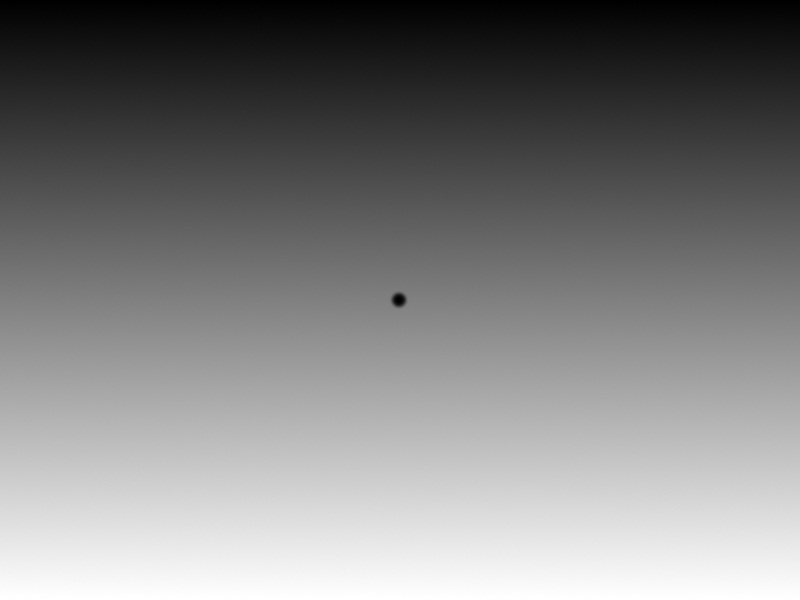
\includegraphics[width=\textwidth]{../data/synth001.jpg}
      \caption{Vertical gray-scale gradient (\emph{grad-vert}).}
      \label{fig:synth-a}
    \end{subfigure}
    ~~
    \begin{subfigure}{0.3\textwidth}
      
\includegraphics[width=\textwidth]{../data/synth002.jpg}
      \caption{Horizontal gray-scale gradient (\emph{grad-hrz}).}
      \label{fig:synth-b}
    \end{subfigure}
    ~~
    \begin{subfigure}{0.3\textwidth}
      
\includegraphics[width=\textwidth]{../data/synth003.jpg}
      \caption{Fine grained noise (\emph{noise-fine}).}
      \label{fig:synth-c}
    \end{subfigure}
  } % makebox

  \makebox[\textwidth][c]{
    \begin{subfigure}{0.3\textwidth}
      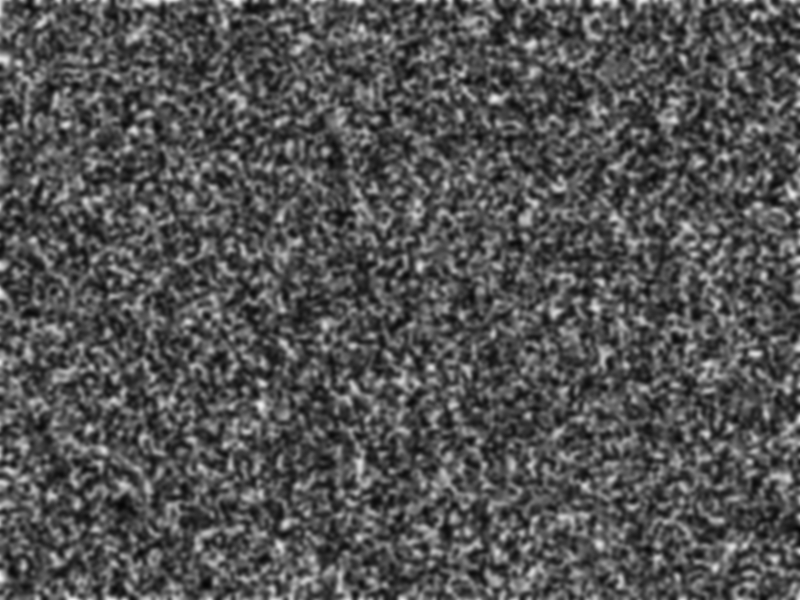
\includegraphics[width=\textwidth]{../data/synth004.jpg}
      \caption{Coarse grained noise (\emph{noise-coarse}).}
      \label{fig:synth-d}
    \end{subfigure}
    ~~
    \begin{subfigure}{0.3\textwidth}
      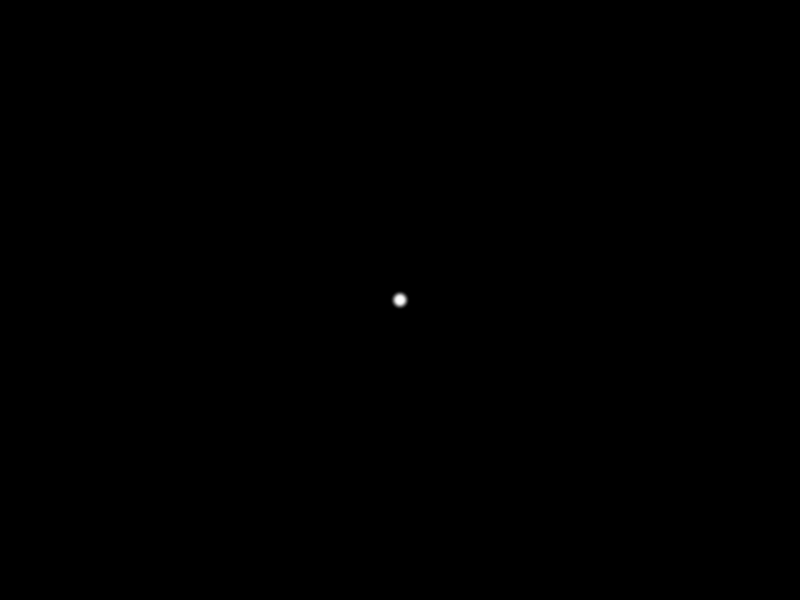
\includegraphics[width=\textwidth]{../data/synth005.jpg}
      \caption{Flat black component (\emph{flat}).}
      \label{fig:synth-e}
    \end{subfigure}
  } % makebox

  \caption[Synthetic input images for area-opening experiments.]{Synthetic input
    images for area-opening experiments. Each image models an extreme case of
    gray-scale image structure.}
  \label{fig:synth}
\end{figure}

\paragraph{Hypothesis 1}

The vertical gradient image in figure~\ref{fig:synth-a} (\emph{grad-vert}) is
supposed to force the sub-image filtering algorithms to work sequentially when
scanning pixels from light to dark. Each thread has to wait until the global
level pointer reaches the level that is within the threads pixel range. While
figure~\ref{fig:synth-b} also consists of a gradient from black to white, the
gradient direction is rotated by 90\degree (\emph{grad-hrz}). The hypothesis is
that sub-image filtering on \emph{grad-vert} is slower than on \emph{grad-hrz},
because there is no expected starvation for the latter, and that, overall,
\emph{grad-vert} is the worst-case for sub-image algorithms. Furthermore, one
can assume that filtering by lines outperforms sub-image filtering in this case.

\paragraph{Hypothesis 2}

Figures~\ref{fig:synth-c} (\emph{noise-fine}) and \ref{fig:synth-d}
(\emph{noise-coarse}) show images generated from random white noise to which a
Gaussian filter has been applied. The granularity of the noise differs, in order
to vary the size of the connected components in the image. We can expect high
performance on both \emph{noise-fine} and \emph{noise-coarse}, since the initial
connectivity is low, when the images are seen as graphs where each pixel is
definitely connected to its neighbors through an edge if the two pixels are at
the same gray level.

\paragraph{Hypothesis 3}

Finally, figure~\ref{fig:synth-e} (\emph{flat}) shows a single, major level
component and therefore has an extremely high connectivity. Based on the results
from section~\ref{sec:experiments-uf-results}, we can expect high contention for
each algorithm, since nearly all pixels are part of the same flat component.

\begin{figure}
  \centering
  \fullmsrow{\synthone}{hypothesis-1-a}
  \caption[Execution time in milliseconds for \emph{grad-vert}.]{Execution time in
    milliseconds for \emph{grad-vert}. In both cases, the performance of sub-image
    filtering algorithms is stable across number of threads.}
  \label{fig:hypothesis-1-a}

  \fullmsrow{\synthtwo}{hypothesis-1-b}
  \caption[Execution time in milliseconds for \emph{grad-hrz}.]{Execution time
    in milliseconds for \emph{grad-hrz}. The optimistic algorithms scale
    negatively with the number of threads, while the STM algorithms remain
    unstable in performance.}
  \label{fig:hypothesis-1-b}

  \fullmsrow{\synththreea}{hypothesis-2-a}
  \caption[Execution time in milliseconds for \emph{noise-fine}.]{Execution time
    in milliseconds for \emph{noise-fine}. The optimistic sub-image filtering
    algorithms improve over the sequential baseline. The STM algorithms run very
    slow in comparison.}
  \label{fig:hypothesis-2-a}
\end{figure}

\begin{figure}[t]
  \centering
  \fullmsrow{\synthfour}{hypothesis-2-b}
  \caption[Execution time in milliseconds for \emph{noise-coarse}.]{Execution
    time in milliseconds for \emph{noise-coarse}. The performance is comparable
    to \emph{noise-fine}.}
  \label{fig:hypothesis-2-b}

  \fullmsrow{\synthfive}{hypothesis-3}
  \caption[Execution time in milliseconds for \emph{flat}.]{Execution time in
    milliseconds for \emph{flat}. The optimistic sub-image filtering algorithms
    outperform the sequential algorithm. Still, the STM algorithms do not come
    close to the sequential baseline.}
  \label{fig:hypothesis-3}
\end{figure}

\subsection{Results and Discussion}
\label{sec:experiments-ao-results}

\subsubsection{Notation and Data Selection}

In this section, I will systematically analyze the results from benchmarking the
different area opening algorithms, based on the hypotheses from
section~\ref{sec:experiments-ao-input-data}. The figures reference the various
algorithms according to table~\ref{tab:algorithms-acronyms}. The only operation
measured is the main-loop of the algorithms. Again, the resolving step is
omitted entirely, mainly because the parallel resolving step would be the same
for all parallel algorithms. For brevity, I will not show and discuss the entire
hypercube of experiments and configurations, and instead present selected
results based on their relevance. After all, we face sixteen different
algorithms -- the algorithms use not only two different variants of shared
union-find, but also different sorting algorithms or shared queues -- and five
different images.

The raw data shows very similar results for \emph{block-counting} and
\emph{block-bucket}, as well as \emph{line-queues-msq} and
\emph{line-queues-array}, respectively, regardless of the underlying data
structures. Therefore, only one configuration of each of these algorithm pairs
is depicted in this section. The raw benchmark results for all algorithms can be
found in appendix~\ref{chpt:omitted-data}. The different queue implementations
only exhibit different performance in the case of \emph{pixel-queues-msq} and
\emph{pixel-queues-array}, which we will discuss in detail in
section~\ref{sec:experiments-ao-results-pixels}.

In this section, the optimistic, fine-grained union-find algorithm is denoted
\emph{opt}, while the STM variant is simply denoted \emph{stm}. If an algorithm
uses any of those algorithms, it is prepended by the according union-find
acronym.

The execution times for all synthetic images and for $\lambda = 3000$ are
shown in figures~\ref{fig:hypothesis-1-a} through \ref{fig:hypothesis-3}. In the
left column, we can see the performance of the optimistic union-find variant,
while on the right, the STM variant's performance is depicted. The legend holds
for each plot of the same column.

\subsubsection{Analysis}

When comparing the performance of optimistic and STM algorithms, it becomes
clear that the STM variants are systematically slower than the optimistic
implementations. This suggests that for practical values of $\lambda$, the
connectivity of the image is not high enough to provoke as much contention as
exhibited in the experiments from section~\ref{sec:experiments-uf-results}. Not
only this, but their performance is developing much more unstable over the
number of hardware threads. This is especially explicit in
figures~\ref{fig:hypothesis-2-a} and \ref{fig:hypothesis-2-b}. None of the STM
variants comes close to the performance baseline of the sequential
algorithm. Because of this obvious infeasibility of the STM algorithms (and for
brevity), I will focus on the analysis of those algorithms that use optimistic
union-find.

\paragraph{Hypothesis 1}

\begin{figure}
  \centering
  \plotrow{\synthone\retries\opt}{Retries for \emph{grad-vert}.}{analysis-hypothesis-1-a}{\synthtwo\cache\opt}{Cache misses for \emph{grad-hrz}.}{analysis-hypothesis-1-b}
  \caption[Performance metrics for \emph{grad-vert} and \emph{grad-hrz}
  (optimistic).]{Performance metrics for \emph{grad-vert} and \emph{grad-hrz}
    (optimistic). The amount of re-tries for sub-image filtering algorithms on
    \emph{grad-vert} is zero, as they are forced to work sequentially. The
    number of cache-misses does not reveal any insights into the negatively
    scaling performance on \emph{grad-hrz}.}
  \label{fig:analysis-hypothesis-1}
\end{figure}

The results, depicted in figure~\ref{fig:hypothesis-1-a}, support the initial
hypothesis that \emph{grad-vert} forces sub-image filtering algorithms to work
in a sequential fashion. The performance of those algorithms is stable over the
number of threads. There are two more observations that require further
analysis.

Firstly, \emph{line-queues-msq} is slower than the already to sequential
performance forced sub-image algorithms. Since the pixel-lines are shared
between threads, the algorithm should encounter less starvation, and therefore
perform faster. The decline in performance is actually due to contention, as we
can see in figure~\ref{fig:analysis-hypothesis-1-a} and due to increased cache
misses (not displayed). Because the threads work sequentially, when performing
sub-image filtering, there is nearly no lock contention on the union-find
roots. In contrast, line-by-line filtering encounters contention already with
only a few threads, as the threads are able to make progress in parallel.

Another interesting observation is that the performance of shared sorting
(\emph{block-counting}) is poor in every exhibited case. This is either due to
contention during sorting, due to starvation when iterating over the shared list
of pixels or even because of conflicts during uniting
pixels. Figure~\ref{fig:analysis-hypothesis-1-a} suggests that the latter is a
major factor.

Secondly, the performance on \emph{grad-hrz} scales negatively with the number
of threads. This is surprising, because the horizontal gradient should provoke
much less starvation than \emph{grad-vert}. The recorded metrics show a linear
increase of cache misses for all algorithms over the number of threads (see
figure~\ref{fig:analysis-hypothesis-1-b}). This alone does not explain the
performance decrease. We will get back to this behavior later in the text.

The hypothesis can only be confirmed partially: \emph{grad-vert} forces
sequential performance as expected, but \emph{grad-hrz} shows decreasing
performance for increasing number of threads. Also, line-based algorithms do not
provide better stability on vertical gradient images.

\paragraph{Hypothesis 2}

Figure~\ref{fig:hypothesis-2-a} and \ref{fig:hypothesis-2-b} support the
hypothesis that, for irregularly structured images, sub-image filter algorithms
excel in performance. Unfortunately, this is still not the case for STM
variants. Again, we can see that the overhead of maintaining single pixel-lines
does not pay off.

The sub-image filter algorithms and the pixel-line based algorithms scale nicely
with the number of threads. Their performance scales effectively up to around
eight threads, from where on no further substantial improvement is visible.

In these cases, even the shared sorting algorithms scale with the number of
available hardware threads. Nevertheless, their performance is still way below
the sequential baseline. We can also see that the STM variants scale according
to the number of threads, but their performance remains unstable and the plots
contain nearly no useful information. However, the hypothesis can be confirmed.

\paragraph{Hypothesis 3}

\begin{figure}
  \centering
  \plotrow{\synthfive\retries\opt}{Number of retries.}{analysis-hypothesis-3-a}{\synthfive\instructions\opt}{Number of issued CPU instructions.}{analysis-hypothesis-3-b}
  \caption[Performance metrics for \emph{flat} (optimistic).]{Performance
    metrics for \emph{flat} (optimistic). The performance of the shared sorting
    algorithm is influenced to a large degree by re-tries and lock contention.}
  \label{fig:analysis-hypothesis-3}
\end{figure}

When filtering a giant connected component, we ought to face high contention, as
shown by the results obtained in
section~\ref{sec:experiments-uf-results}. Surprisingly, the results shown in
figure~\ref{fig:hypothesis-3} show only a serious performance decrease for
\emph{block-counting}. The metrics displayed in
figure~\ref{fig:analysis-hypothesis-3} show that the number of instructions
increases nearly linearly with the number of hardware threads, while the number
of retries is consistently high.

On the other hand, the sequential and sub-image filtering algorithms excel in
this case. The pixel-line based algorithm does not show any performance
increase, but also no decline. The giant connected component seems not to have
any effect on the performance, which is comparable to the optimal case
(i.e. \emph{noise-fine} and \emph{noise-coarse}). This is surprising, as it
directly contradicts the notion that large connected components cause
contention. Neither the number of retries, nor the number of issued instructions
increases to any noticeable degree.

This suggests that there is few overlap between the single threads when
filtering sub-images. The starting indices of the independent threads are
located ``far away'' from each other (recall the sub-image filtering algorithms
described in sections~\ref{sec:area-opening-no-sorting-sub-image} and
\ref{sec:area-opening-local-sorting-sub-image}). Therefore, increased contention
only becomes an issue very late in the filtering process, as soon as threads
begin to unite connected components across sub-image borders. Since this is only
a small fraction of work compared to building the thread-local connected
components, its impact on the performance is minimal.

The hypothesis holds for some of the parallel area opening algorithms but cannot
be confirmed completely. The structure of the sub-image filtering algorithms
counters the effect of a giant connected component. This also suggests an
explanation for why the performance on \emph{grad-hrz} was unexpectedly
bad for sub-image filtering: since the level components on
\emph{grad-hrz} are ordered horizontally and extend across all sub-image
borders, contention is encountered very early, as each thread repeatedly tries
to unite its connected component with those of other threads already in the
beginning, so that all threads work on the same connected component, which is
therefore locked frequently.

\subsection{Pixel Queues}
\label{sec:experiments-ao-results-pixels}

\begin{figure}
  \centering
  \areaopenplotpixels
  \caption[Benchmark results for \emph{pixel-queue} variants on
  \emph{noise-coarse}.]{Benchmark results for \emph{pixel-queue} variants on
    \emph{noise-coarse}. The execution time is extremely high for each
    variant. The sequential performance baseline is barely visible.}
  \label{fig:pixel-queues}
\end{figure}

The results for pixel queue algorithms are special in terms of performance and
therefore, I devote a separate section to those. Figure~\ref{fig:pixel-queues}
displays the benchmark metrics for experiments on image \emph{noise-coarse}. For
the experiments, the image has been scaled down to $800 \times 600$ pixels, in
order to reduce the overall testing time. We can see from
figure~\ref{fig:pixel-queues-ms} that the performance of \emph{all} variants of
\emph{pixel-queues} is dramatically worse, especially with regard to the number
of hardware threads, than the base-line performance of the sequential algorithm.

Even though we can expect slow performance because of the missing sorting of
pixels, the results are surprising. The naive sub-image filtering algorithm,
which also operates in $O(kn)$, exceeds the sequential algorithm in
performance. Executing \emph{pixel-queues} algorithms, as described in
section~\ref{sec:experiments-microbenchmarks}, on a single image took in
practice about a day for all combinations of parameters. It is especially
interesting to investigate the reasons for this.

Here, both union-find variants behave very similarly for all metrics. We can
therefore already conclude that this is not a union-find based problem. Instead,
the different queue implementations seem to suffer heavily from high
throughput. The conflicts handled by the union-find implementations do not
increase together with the elapsed measured time. Therefore, even though
union-find conflicts might be responsible for the initial increase, they are not
the reason for the overall dramatic performance.

Instead, each queue data structure suffers from a different
phenomenon. Figure~\ref{fig:pixel-queues-cache-misses} shows how the number of
cache misses increases already when using only two threads for the bounded array
queue, probably due to false sharing \cite{Bolosky1993False}. False sharing
describes an effect caused by cache coherence protocols on shared memory
processors. Each processor has its own cache, which contains copies of the data
of the other processors' caches. When a processor writes a word into one of the
cache lines of its local cache, the entire cache line gets invalidated for all
other processors. Consequently, all other caches need to update this line. This
happens especially often, if more than one independent word is stored per cache
line, so that many words are falsely invalidated \cite{Bolosky1993False}. In
many cases, this invalidation would be unnecessary and it therefore results in a
slow down of the processors \cite{Bolosky1993False}. Notice how the shape of the
plot for the bounded array queue in figure~\ref{fig:pixel-queues-cache-misses}
resembles the one in figure~\ref{fig:pixel-queues-ms}.

The \citet{Anderson1994Waitfree} queue exhibits no false sharing. The reason for
its poor performance is depicted in
figure~\ref{fig:pixel-queues-instructions}. The more threads at this high level
of throughput are used, the more conflicts are encountered. Therefore, the
number of issued instructions increases with the number of threads.

Based on these results, we can conclude that using complex data structures to
maintain sole pixels, proves not to be a reliable technique for area
opening. Not only the overhead of adding and removing each pixel many times from
a queue, but also the described false sharing, make this type of algorithm
unfeasible.

\subsection{Natural Images}
\label{sec:experiments-ao-nat}

\newcommand{\rbc}{\emph{rbc}}
\newcommand{\facade}{\emph{facade}}
\newcommand{\mammo}{\emph{mammo}}

\begin{figure}
  \centering

  \makebox[\textwidth][c]{
    \begin{subfigure}{0.3\textwidth}
      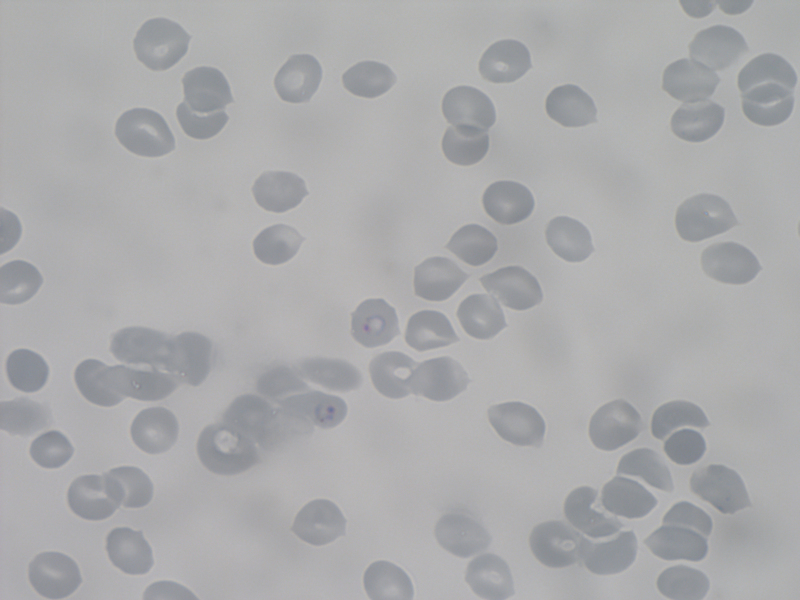
\includegraphics[width=\textwidth]{../data/natural001.jpg}
      \caption{Red blood cells infected with Malaria parasites (\emph{rbc}), $1600
        \times 1200$ pixels.}
      \label{fig:nat-a}
    \end{subfigure}
    ~
    \begin{subfigure}{0.3\textwidth}
      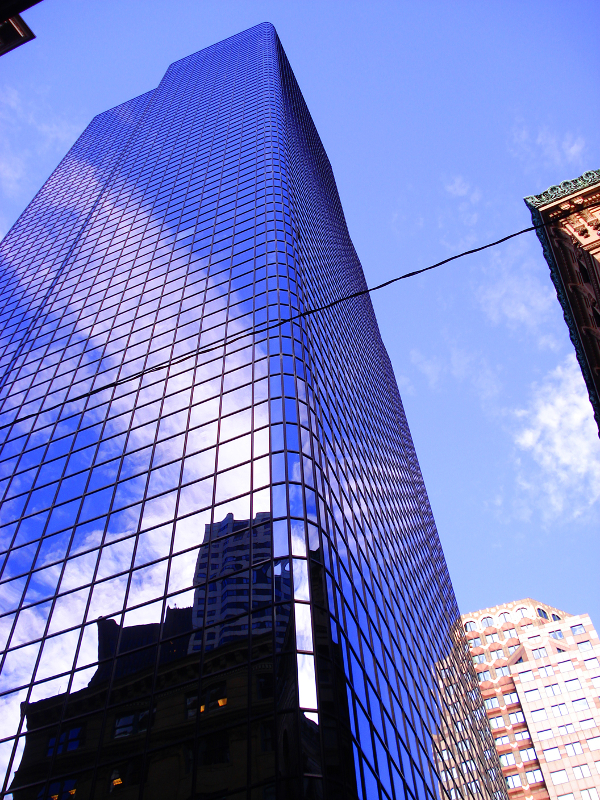
\includegraphics[width=\textwidth]{../data/natural002.jpg}
      \caption{Facade of an office building (\emph{facade}), $600 \times 800$ pixels.}
      \label{fig:nat-b}
    \end{subfigure}
    ~
    \begin{subfigure}{0.3\textwidth}
      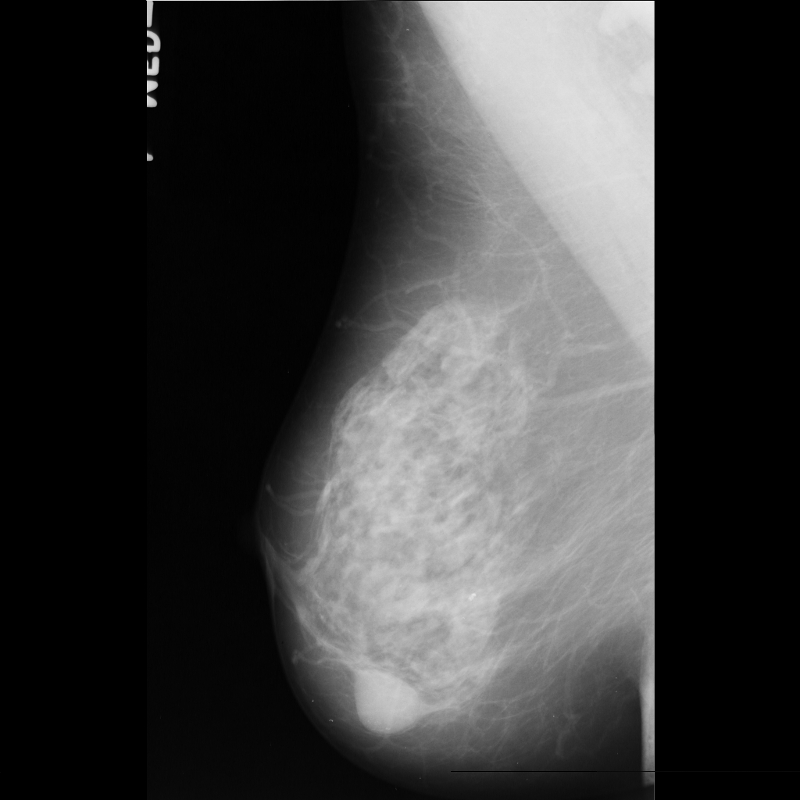
\includegraphics[width=\textwidth]{../data/natural003.jpg}
      \caption{Mammography scan (\emph{mammo}), $800 \times 800$ pixels.}
      \label{fig:nat-c}
    \end{subfigure}
  } % makebox

  \caption[Natural input images for area-opening experiments.]{Natural input
    images for area-opening experiments. The images represent different
    real-life use cases of morphological area opening.}
  \label{fig:nat}
\end{figure}

\begin{figure}
  \centering
  \plotsingle
  {\natone\ms\opt}
  {Results for \emph{rbc}.}
  {nat-results-a}

  \plotrow
  {\nattwo\ms\opt|pixel}
  {Results for \emph{facade}.}
  {nat-results-b}
  {\natthree\ms\opt|pixel}
  {Results for \emph{mammo}.}
  {nat-results-c}
  \caption[Execution time in milliseconds for natural images using optimistic
  union-find.]{Execution time in milliseconds for natural images using
    optimistic union-find. It becomes clear that there is a lower bound on the
    image size with regard to speedup. Also, there is an upper bound on number
    of threads, as in most cases, the performance declines around eight
    threads.}
  \label{fig:nat-results}
\end{figure}

To validate the results against real life input, we will concern three realistic
cases of natural images, which can be analyzed using morphological area opening
in various forms. The images are displayed in figure~\ref{fig:nat}. Due to being
captured by different means, the dimensions of these images vary. All images
were converted to 8-bit gray-scale.

Figure~\ref{fig:nat-a} shows a blood sample Malaria parasites
(\emph{rbc}). The photography in figure~\ref{fig:nat-b} shows the facade of an
office building (\emph{facade}). In figure~\ref{fig:nat-c}, we see a mammography
scan of a female breast (\emph{mammo}), which has been obtained from \emph{The
  Mammographic Image Analysis Society digital mammogram database}
\cite{Suckling1994Mammographic}.

The benchmark results for the natural images are displayed in
figure~\ref{fig:nat-results}. It is easy to see that the behavior of the
algorithms on natural images closely resembles the results obtained on synthetic
images. These plots also make it very clear, that there is a lower bound on the
image size, that needs to be taken into account, in order to gain any
performance increase by using parallel area opening.

Also, there is an upper bound on the number of threads with regard to
performance in the majority of cases. We see in both figures that the, already
encountered, upper bound on threads seems to be a pattern. The performance
declines around eight threads (see again figures~\ref{fig:nat-results-b} and
\ref{fig:nat-results-c}). This might be due to a larger number objects crossing
sub-image borders on natural images.

The results for \emph{rbc} (figure~\ref{fig:nat-results-a}) closely resemble the
results for fine grained synthetic noise images,
i.e. figure~\ref{fig:hypothesis-2-a}. The performance on \emph{facade} and
\emph{mammo} (figures~\ref{fig:nat-results-b} and \ref{fig:nat-results-c}) is
comparable to the results shown in figure~\ref{fig:hypothesis-2-b} with a twist:
the natural input images have smaller dimensions and the algorithms, at no time,
outperform sequential area opening. We can conclude that this is due to the
input image size and that it therefore does not pay off to filter small images
(i.e. $800 \times 600$ pixels) using parallel area opening.

\subsection{Scaling Behavior for $\lambda$}
\label{sec:experiments-ao-scale}

There is one more parameter, which we did not yet address. The size of $\lambda$
has an effect on the size of connected components: it is the upper bound on size
for non-level pixel components (see section~\ref{sec:morphology-area-opening})
and therefore potentially influences lock contention. If the structure of the
image only allows for components smaller than $\lambda$, or, if the image
exhibits a large number of flat level components, its effect is countered.

Experiments on \emph{noise-fine} suggest that practical values of $\lambda$ do
not have any immediate effect on sub-image filtering algorithms (see results in
figure~\ref{fig:scale-results}). Also, he sequential base-line does not change
with increased $\lambda$. This is actually true for differently structured
images as well, if we take the results presented in
section~\ref{sec:experiments-ao-results} into account.

The parallel algorithms do not behave equally for increased values of
$\lambda$. There is a slight performance drop exhibited by
\emph{block-counting}. Since its performance already is poor, the changes are
barely noticeable. Different so for line-based filtering. By comparing
figure~\ref{fig:scale-results-6000} to figure~\ref{fig:scale-results-9000}, it
becomes obvious that the line-based algorithm does indeed suffer from increased
$\lambda$. The sub-image filtering algorithms, however, exhibit constant
performance for increased $\lambda$, which is a clear advantage.

We can conclude that, for practical values of $\lambda$, its effect on the
performance of the sub-image algorithms is negligible in comparison to image
structure. This is supported by the experimental results presented by
\citet{Meijster2002Comparison}, which indicate no dependency of the performance
of union-find area opening in relation to $\lambda$. Therefore, optimistic
sub-image filtering with thread-local sorting is not only the fastest, but also
the most robust parallel algorithm for area opening.

\begin{figure}
  \centering
  \plotrow{\synththreeb\ms\opt}{}{scale-results-6000}{\synththreec\ms\opt}{}{scale-results-9000}
  \caption[Benchmark results for \emph{noise-fine} and increasing $\lambda$
  using optimistic union-find.]{Benchmark results for \emph{noise-fine} and
    increasing $\lambda$ using optimistic union-find. Sub-image filtering
    algorithms are not affected by increasing values of $\lambda$, but
    line-based and shared-sorting variants react with declining performance.}
  \label{fig:scale-results}
\end{figure}

%%% Local Variables:
%%% mode: latex
%%% TeX-master: "main"
%%% End:


\chapter{Discussion}
\label{chpt:discussion}

\section{Contributions}
\label{sec:discussion-contribution}

As a major result, we can conclude, from the findings made in
section~\ref{sec:experiments-area-opening}, that sub-image area opening with
thread-local sorting, using a fine-grained optimistic locking scheme for the
union-find implementation, is the most efficient and robust parallel algorithm
presented in this thesis.

Model checking, as shown in chapter~\ref{chpt:correctness}, showed that the
parallel algorithm compute the same result as the sequential algorithm by
\citet{Meijster2002Comparison}. It benefits from an inherent heuristic, which is
an expectable large distance between the pixel start indices on the image array
for the independent threads. Therefore, lock contention on single trees is low
in most of the cases. There are two cases, however, which pose worst case
scenarios to the algorithm. These are image gradients in $x$- or $y$-direction,
which dominate the image structure. In these cases, the algorithm is either (1)
forced to work in a sequential fashion, which is slower than the sequential
baseline, due to the threading overhead, or (2) encounters high lock contention,
due to level components extending excessively across sub-image borders.

It is interesting to see that parallel algorithms with the same formal
complexity behave very differently in practice. For example, the shared sorting
algorithms, which run in $O(k + n)$, do not perform well in any case, while the
most naive algorithm in $O(kn)$ (that is, sub-image filtering without sorting)
is second to best in every experiment.

Effects such as false sharing \cite{Bolosky1993False} and lock contention have a
huge influence on the actual performance. So does the input structure, apart
from its size, as we saw in the results obtained by independent union-find
experiments, shown in section~\ref{sec:experiments-uf-results}. Here, the
connectivity of the input graph made a large difference in terms of performance.

A similar algorithm for labeling connected flat components on gray-scale images,
based on union-find was proposed by \citet{Hesselink2001Concurrent}. The
algorithm they proposed does \emph{not} compute area opening, which is the major
difference to this thesis. Their approach uses no shared union-find data
structure, but a message passing system through which ownership of disjoint sets
is moved between threads. This means that Hesselink et al.'s approach does not
benefit from implicitly shared data structures. Still, their results show that
their algorithm scales linearly with the number of hardware threads. Even though
their algorithm and the ones developed in this thesis are closely related, they
are only comparable to some degree.

Sub-image parallel area opening, in its current version, does not scale linearly
with the number of hardware threads. In the presented experimental results, it
first begins to show a noticeable improvement over the sequential algorithm when
running on four threads, and already stops improving at around eight to ten
threads. This upper bound will presumably increase with the size of the
input. Nevertheless, this also means that, in order to gain a substantial
performance improvement, we need to provide the algorithm with a sufficiently
large image to filter. This suggests that the sequential algorithm by
\citet{Meijster2002Comparison} already performs optimally.

The number of algorithms developed in this thesis is comparably large in order
to give a comprehensive overview over efficient parallelization strategies for
area opening. Knowing which algorithms yield good performances, only analyzing a
few of those with less parameters (i.e. parallel union-find variants, different
implementations of auxiliary data structures, etc.) will provide further
interesting insights.

\section{Future Work}
\label{sec:future-work}

Taken the insights found in this thesis, there are quite a number of
possibilities for further research directions and implementation work. For
example, a more remote task would be bug-fixing and extending JPF to be able to
fully model check the presented algorithms.

In order to perform a more general verification of area opening algorithms, it would be
helpful to find the ``sweet spot'' between operational correctness conditions,
as presented in section~\ref{sec:correctness-area-opening-properties-ao}, and
black-box testing conditions, as shown in
section~\ref{sec:correctness-experimental}. This could help to identify and
verify even more efficient parallel area opening algorithms and also to verify
generalizations of parallel area opening. Such properties should also focus more
on consistency. A node's parent value is invariant as soon as it is equal or
greater to zero, so that $I: ~ 0 \leq \inlinecode{parent(find(x))}$ and $\{I\} ~
c ~ \{I\}$, where $c$ is any function defined in
section~\ref{sec:morphology-algorithm}.  This invariant implies the absence of
deletion in the union-find data structure and should be part of an extended
formal validation of parallel area opening to ensure consistency.

As already pointed out, there exists a generalized variant of area opening,
namely morphological attribute opening \cite{Breen1996Attribute}. The sub-image
area opening algorithm could, in principle, easily be extended to attribute
openings, as done by \citet{Wilkinson2000Fast} for the sequential algorithm
\cite{Meijster2002Comparison}. Additionally, \citet{Meijster2001Fast} showed
that union-find based area opening can directly be projected onto the
computation of area granulometry, or area pattern spectra
\cite{Meijster2002Comparison}. Area pattern spectra are histograms of the size
distribution over a given image \cite{MohanaRao2001Areagranulometry}. Computing
these spectra is helpful in order to estimate the average size of elements that
are expected to pose the majority of an image for further segmentation.

It would be interesting to assess the performance of sub-image parallel area
opening more deeply. In order to avoid the issues of micro benchmarks in managed
languages like Java, one could re-implement the algorithm in a medium-level
language, such as C or C{}\verb!++!. Additionally, the algorithm could be
extended to also filter 3D voxel images. Based on the findings that large images
benefit more from the parallel algorithms, the performance on three dimensional
data can be expected to be very fast. Furthermore, the performance of sub-image
parallel area opening should be compared systematically to the performance of
parallel Max-Tree computation \cite{Wilkinson2008Concurrent}.

Also, the number of regional maxima on images could then be controlled to a
greater extend, for example by controlling the number of level components
explicitly, and there would be more room for more exhaustive performance
experiments.

Furthermore, the sub-image filtering algorithm needs to be stabilized against
worst case image scenarios. One approach could be to simply use the sequential
algorithm in such cases, based on a heuristic analysis of the image
structure. Analyzing the image entirely once, and then filtering it, is, on
average, probably just as slow as always simply running the parallel
algorithm. Instead, one could examine how the image can be split up between
threads, as to avoid sub-image patterns, which are prone to contention with
regard to image structure. For example, instead of defining intervals on the
pixel array, in which each thread may access pixels, one could assign a
rectangle of pixels to each thread that is also limited on the $x$ axis.

Lastly, one should mention that modern GPUs provide a fast platform for parallel
image algorithms and it is therefore tempting to think about an area opening
algorithm for GPUs. An approach to implementing sub-image parallel area opening
on GPUs could be a union of the algorithm presented in this thesis and the
cross-thread message passing union-find algorithm for flat component labeling,
as presented by \citet{Hesselink2001Concurrent}.

%%% Local Variables:
%%% mode: latex
%%% TeX-master: "main"
%%% End:


\chapter{Conclusion}
\label{chpt:conclusion}

In this thesis, I presented a variety of parallel algorithms to compute
morphological area opening based on the sequential, union-find based algorithm
by \citet{Meijster2002Comparison}. In particular, one of these parallel
algorithms -- namely parallel sub-image area opening with thread local pixel
sorting, which is based on a concurrent union-find data structure, that uses a
fine-grained locking scheme -- proved to outperform the sequential algorithm on
irregularly structured and flat images. Nevertheless, there exist at least two
pathological cases of input images, which let the performance of the new
parallel algorithm deteriorate. Future work should aim at finding a solution to
this. Additionally, I defined formal correctness conditions and showed that
model checking the new, parallel area opening algorithms through Java Pathfinder
\cite{Visser2003Model} does not reveal any errors. JPF identified bugs in
deliberately buggy implementations, which suggests that the here developed
algorithms are correct.

Furthermore, I provided a detailed discussion of the original sequential
algorithm, as well as its formalization and examples of its filtering effect on
images. Additionally, I identified parallel union-find algorithms that can be
mapped to area opening. The various union-find algorithms have been examined in
detail and their performance has been assessed independently on differently
structured input graphs. This showed that wait-free union-find and a mixed
wait-free and STM union-find algorithm outperform optimistic, fine-grained
locking union-find on graphs of high connectivity, since lock contention on a
single giant connected component is simply too high.

In contrast to this, we saw that these limitations do not necessarily apply to
parallel sub-image area opening, because here, each thread starts its work on
pixels on the image, which, on the array of image pixels, are located ``far
away'' from each other. Extensive lock contention is limited to a small portion
of work at the end of the filtering process. In the case of parallel area
opening, STM implementations of union-find exhibit systematically lower
performance. This might be due to the chosen STM library and further research on
this is needed.

This thesis opens up for many future research directions. While some of these
suggestions focus on validation and extension of the results presented in this
thesis, others focus on technical improvements. I believe that both are highly
relevant for parallel area opening to become a fast and reliable tool for use in
image analysis.

%%% Local Variables:
%%% mode: latex
%%% TeX-master: "main"
%%% End:


\bibliographystyle{unsrtnat}
\bibliography{thesis.bib}

\appendix

\chapter{Auxiliary Algorithms}
\label{chpt:auxiliary-algorithms}

\section{Bounded Array Queue}
\label{sec:bounded-array-queue}

The implementation of the bounded array queue, which I use for maintaining work
items like pixels or image lines, is lock-free. It maintains two instances of
\inlinecode{AtomicInteger}, that point to the \inlinecode{head} and the
\inlinecode{tail} of the queue (i.e. indices on the pixel array). The array is
always of size $2^n$. This makes it possible to use the bit-wise \emph{and}
operator to compute modulo of the \inlinecode{head} and \inlinecode{tail}
pointers, in order to wrap-around the pointers to point to the beginning of the
underlying array again. The queue is empty, if \inlinecode{head} =
\inlinecode{tail}. When an element is enqueued, \inlinecode{tail} is advanced,
pointing to the next empty array index. When fetching an element from the queue,
\inlinecode{head} is advanced again. Each of these operations has a complexity
of constant time. The implementation of these functions is shown in detail in
figure~\ref{fig:bounded-array-queue}. For brevity, the constructor and other,
rather uninteresting, details are omitted.

\begin{figure}
  \centering
  \lstinputlisting[linerange={queue0-queue1,queue2-queue3,queue4-queue5,queue6-queue7,queue8-queue9}]{../parallel-morphology/src/dk/itu/parallel/morphology/util/queues/ConcurrentArrayQueue.java}
  \caption{The implementation of the bounded array queue.}
  \label{fig:bounded-array-queue}
\end{figure}

\section{Shared Queues}
\label{sec:area-opening-queues} % kept like this to not break references

\begin{figure}
  \centering

  \lstinputlisting[linerange={queues0-queues1,queues2-queues3,queues4-queues5}]{../parallel-morphology/src/dk/itu/parallel/morphology/util/queues/Queues.java}

  \caption{The \inlinecode{Queues} container class.}
  \label{fig:ao-wf-queues}
\end{figure}

The \inlinecode{Queues} data structure maintains two concurrent queues,
\inlinecode{upper} and \inlinecode{lower}, and a level pointer which indicates
the currently filtered gray-scale level. On initialization, all items are
enqueued to \inlinecode{upper}. Calling \inlinecode{pop}, the upper queue is
successively emptied by consuming threads. After the threads are done with their
work on the retrieved item, they put it into the lower queue through
\inlinecode{enqueue}.

Atomically swapping and gray-level decrease is implemented in the auxiliary
function \inlinecode{swapAndDecrement}. Each thread acquires a local reference
of the thread global \inlinecode{Queues} instance. It can then issue a call to
update the global queue, using its local reference to check if it is up to date:

\lstinputlisting[style=inline, linerange={swap0-swap1}]{../parallel-morphology/src/dk/itu/parallel/morphology/util/queues/Queues.java}

Obviously, the swap will fail if the calling thread does not have the most
recent information on the global queues stored locally, so that we can make sure
that it will be swapped only once per level.

\section{Pixel Line Representation}
\label{sec:pixel-line}

\begin{figure}
  \centering
  \lstinputlisting[linerange={line0-line1}]{../parallel-morphology/src/dk/itu/parallel/morphology/filter/QueueLines.java}

  \caption{The \inlinecode{Line} container class implementation.}
  \label{fig:line-class}
\end{figure}

In order to represent a single pixel line, we rely on a container class
\inlinecode{Line}, that wraps an array, which in turn contains, by gray-scale
value sorted, pixel indices. For convenience, the container class also
internally maintains a pointer to the pixel, which will be returned on the next
call to \inlinecode{current}. Furthermore, the function \inlinecode{advance}
moves the pointer and returns true, if the internal pointer is not yet outside
of the array bounds. The same check can be performed by calling
\inlinecode{workLeft}. The entire implementation is depicted in
figure~\ref{fig:line-class}.

\chapter{Raw Data Plots}
\label{chpt:omitted-data}

\begin{figure}[h]
  \centering
  \fullrawrow{\synthone}{ms}{raw-hypothesis-1a}
  \caption{Execution time in miliseconds for \emph{grad-vert}.}
  \fullrawrow{\synthone}{retries}{raw-hypothesis-1a}
  \caption{Number of retries for \emph{grad-vert}.}
\end{figure}

\begin{figure}
  \centering
  \fullrawrow{\synthone}{cache-misses}{raw-hypothesis-1a}
  \caption{Number of cache-misses for \emph{grad-vert}.}
  \fullrawrow{\synthone}{instructions}{raw-hypothesis-1a}
  \caption{Number of issued CPU instructions for \emph{grad-vert}.}
  \fullrawrow{\synthtwo}{ms}{raw-hypothesis-1b}
  \caption{Execution time in milliseconds for \emph{grad-hrz}.}
\end{figure}

\begin{figure}
  \centering
  \fullrawrow{\synthtwo}{retries}{raw-hypothesis-1b}
  \caption{Number of retries for \emph{grad-hrz}.}
  \fullrawrow{\synthtwo}{cache-misses}{raw-hypothesis-1b}
  \caption{Number of cache-misses for \emph{grad-hrz}.}
  \fullrawrow{\synthtwo}{instructions}{raw-hypothesis-1b}
  \caption{Number of issued CPU instructions for \emph{grad-hrz}.}
\end{figure}

\begin{figure}
  \centering
  \fullrawrow{\synththreea}{ms}{raw-hypothesis-2a}
  \caption{Execution time in miliseconds for \emph{noise-fine}.}
  \fullrawrow{\synththreea}{retries}{raw-hypothesis-2a}
  \caption{Number of retries for \emph{noise-fine}.}
  \fullrawrow{\synththreea}{cache-misses}{raw-hypothesis-2a}
  \caption{Number of cache-misses for \emph{noise-fine}.}
\end{figure}

\begin{figure}
  \centering
  \fullrawrow{\synththreea}{instructions}{raw-hypothesis-2a}
  \caption{Number of issued CPU instructions for \emph{noise-fine}.}
  \fullrawrow{\synthfour}{ms}{raw-hypothesis-2b}
  \caption{Execution time in miliseconds for \emph{noise-coarse}.}
  \fullrawrow{\synthfour}{retries}{raw-hypothesis-2b}
  \caption{Number of retries for \emph{noise-coarse}.}
\end{figure}

\begin{figure}
  \centering
  \fullrawrow{\synthfour}{cache-misses}{raw-hypothesis-2b}
  \caption{Number of cache misses for \emph{noise-coarse}.}
  \fullrawrow{\synthfour}{instructions}{raw-hypothesis-2b}
  \caption{Number of issued CPU instructions for \emph{noise-coarse}.}
  \fullrawrow{\synthfive}{ms}{raw-hypothesis-3}
  \caption{Execution time in miliseconds for \emph{flat}.}
\end{figure}

\begin{figure}
  \centering
  \fullrawrow{\synthfive}{retries}{raw-hypothesis-3}
  \caption{Number of retries for \emph{flat}.}
  \fullrawrow{\synthfive}{cache-misses}{raw-hypothesis-3}
  \caption{Number of cache misses for \emph{flat}.}
  \fullrawrow{\synthfive}{instructions}{raw-hypothesis-3}
  \caption{Number of issued CPU instructions for \emph{flat}.}
\end{figure}

\begin{figure}
  \centering
  \fullrawrow{\natone}{ms}{raw-nat-1}
  \caption{Execution time in miliseconds for \emph{rbc}.}
  \fullrawrow{\natone}{retries}{raw-nat-1}
  \caption{Number of retries for \emph{rbc}.}
  \fullrawrow{\natone}{cache-misses}{raw-nat-1}
  \caption{Number of cache misses for \emph{rbc}.}
\end{figure}

\begin{figure}
  \centering
  \fullrawrow{\natone}{instructions}{raw-nat-1}
  \caption{Number of issued CPU instructions for \emph{rbc}.}
  \fullrawrownat{\nattwo}{ms}{raw-nat-2}
  \caption{Execution time in miliseconds for \emph{facade}.}
  \fullrawrownat{\nattwo}{retries}{raw-nat-2}
  \caption{Number of retries for \emph{facade}.}
\end{figure}

\begin{figure}
  \centering
  \fullrawrownat{\nattwo}{cache-misses}{raw-nat-2}
  \caption{Number of cache misses for \emph{facade}.}
  \fullrawrownat{\nattwo}{instructions}{raw-nat-2}
  \caption{Number of issued CPU instructions for \emph{facade}.}
  \fullrawrownat{\natthree}{ms}{raw-nat-3}
  \caption{Execution time in miliseconds for \emph{mammo}.}
\end{figure}

\begin{figure}
  \centering
  \fullrawrownat{\natthree}{retries}{raw-nat-3}
  \caption{Number of retries for \emph{mammo}.}
  \fullrawrownat{\natthree}{cache-misses}{raw-nat-3}
  \caption{Number of cache misses for \emph{mammo}.}
  \fullrawrownat{\natthree}{instructions}{raw-nat-3}
  \caption{Number of issued CPU instructions for \emph{mammo}.}
\end{figure}

%%% Local Variables:
%%% mode: latex
%%% TeX-master: "main"
%%% End:


\end{document}
